% file: HrdwCCppCUDA.tex
%
% github        : ernestyalumni
% gmail         : ernestyalumni 
% linkedin      : ernestyalumni 
% wordpress.com : ernestyalumni
%
% This code is open-source, governed by the Creative Common license.  Use of this code is governed by the Caltech Honor Code: ``No member of the Caltech community shall take unfair advantage of any other member of the Caltech community.'' 

\documentclass[10pt]{amsart}
\pdfoutput=1
\usepackage{mathtools,amssymb,caption}

\usepackage{graphicx}
\usepackage{hyperref}
\usepackage[utf8]{inputenc}
\usepackage{listings}
\usepackage[table]{xcolor}
\usepackage{pdfpages}
\usepackage{tikz}
\usetikzlibrary{matrix,arrows,backgrounds}

\usepackage{breqn} % for dmath


%\usepackage{cancel} % for Feynman slash notation

\hypersetup{colorlinks=true,citecolor=[rgb]{0,0.4,0}}


%\oddsidemargin=15pt
%\evensidemargin=5pt
%\hoffset-45pt
%\voffset-55pt
%\topmargin=-4pt
%\headsep=5pt
%\textwidth=1120pt
%\textheight=595pt
%\paperwidth=1200pt
%\paperheight=700pt
%\footskip=40pt








\newtheorem{theorem}{Theorem}
\newtheorem{corollary}{Corollary}
%\newtheorem*{main}{Main Theorem}
\newtheorem{lemma}{Lemma}
\newtheorem{proposition}{Proposition}

\newtheorem{definition}{Definition}
\newtheorem{remark}{Remark}

\newenvironment{claim}[1]{\par\noindent\underline{Claim:}\space#1}{}
\newenvironment{claimproof}[1]{\par\noindent\underline{Proof:}\space#1}{\hfill $\blacksquare$}

%This defines a new command \questionhead which takes one argument and
%prints out Question #. with some space.
\newcommand{\questionhead}[1]
  {\bigskip\bigskip
   \noindent{\small\bf Question #1.}
   \bigskip}

\newcommand{\problemhead}[1]
  {
   \noindent{\small\bf Problem #1.}
   }

\newcommand{\exercisehead}[1]
  { \smallskip
   \noindent{\small\bf Exercise #1.}
  }

\newcommand{\solutionhead}[1]
  {
   \noindent{\small\bf Solution #1.}
   }


  \title[Hardware (Compilers, OS, runtime) and C, C++, to CUDA]{Hardware (Compilers, OS, runtime) and C, C++, to CUDA}

\author{Ernest Yeung \href{mailto:ernestyalumni@gmail.com}{ernestyalumni@gmail.com}}
\date{1 Nov 2017}
\keywords{C, C++, CUDA, CUDA C/C++, Compilers, OS, runtime, classes, Object Oriented Programming, Segmentation Fault, memory, memory addresses}

\begin{document}

\definecolor{darkgreen}{rgb}{0,0.4,0}
\lstset{language=Python,
 frame=bottomline,
 basicstyle=\scriptsize,
 identifierstyle=\color{blue},
 keywordstyle=\bfseries,
 commentstyle=\color{darkgreen},
 stringstyle=\color{red},
 }
%\lstlistoflistings

\maketitle

\tableofcontents

\begin{abstract}
I review what, how, and why Segmentation Fault is and occurs in the specific context of C and hopefully to CUDA, virtual memory addresses in C++, and to CUDA.  


\end{abstract}

\section{Introduction; why I'm writing this}  

I didn't realize the importance of having a profound understanding of C/C++ and its relation to hardware, in particular memory (addresses), until I learned more specifically about the work done at NVIDIA from its news and job postings.  Coming from a theoretical and mathematical physics background, I wanted to get myself up to speed as fast as possible, provide good textbook and online references, and directly relate these topics, which seem to be classic topics in computer science (at hardware level) and electrical engineering, to CUDA, to specifically GPU parallel programming with direct CUDA examples.  

Note that there is a version of this LaTeX/pdf file in a "grande" format (not letter format but "landscape" format) that is exactly the same as the content here, but with different size dimensions.  


I began looking up resources (books, texts, etc.) \href{https://softwareengineering.stackexchange.com/questions/127101/recommend-a-text-that-explains-the-physical-implementation-of-c-stack-heap-et}{Recommend a text that explains the physical implementation of C (stack, heap, etc) [closed]}, and a \href{https://softwareengineering.stackexchange.com/users/39294/dipan-mehta}{Mehta} recommended books including Hyde (2006) \cite{Hyde2006}.  

\begin{quotation}
	"When programmers first began giving up assembly language in favor of using HLLs, they generally understood the low-level ramifications of the HLL statements they were using and could choose their HLL statements appropriately.Unfortunately, the generation of computer programmers that followed them did not have the benefit of mastering assembly language. As such, they were not in a position to wisely choose statements and data structures that HLLs could efficiently translate into machine code."  
\end{quotation}
pp. 2, Ch. 1 of Hyde (2006) \cite{Hyde2006}, where HLL stands for high-level language.  I was part of that generation and knew of nothing of assembly.  

\section{80x86 Assembly; 80x86 Architecture}  

cf. Ch. 3 of Hyde (2006) \cite{Hyde2006}

Main difference between complex instruction set computer (CISC) architectures such as 80x86 and reduced instruction set computer (RISC) architectures like PowerPC is the way they use memory.  RISC provde relatively clumsy memory access, and applications avoid accessing memory.  80x86 access memory in many different ways and applications take advantage of these facilities.  

\subsection{Basic 80x86 Architecture}  

Intel CPU generally classified as a \emph{Von Neumann machine}, containing 3 main building blocks:
\begin{enumerate}
	\item CPU
	\item memory
	\item input/output (I/O) devices
\end{enumerate}
These 3 components are connected together using the \emph{system bus}.  System bus consists of 
\begin{itemize}
	\item address bus
	\item data bus
	\item control bus
\end{itemize}

CPU communicates with memory and I/O devices by placing a numeric value on the address bus to select 1 of the memory locations or I/O device port locations, each of which has a unique binary numeric address.   \\
Then the CPU, I/O, and memory devices pass data among themselves by placing data on the data bus.   \\
Control bus contains signals that determine the direction of data transfer (to or from memory, and to or from an I/O device).  

So 
\[
\begin{gathered}
\begin{gathered}
\textbf{Memory} \\
\text{Obj}{(\textbf{Memory})} = \text{ memory locations } 
\end{gathered} \\ 
\begin{gathered}
\textbf{I/O} \\
\text{Obj}{(\textbf{I/O})} = \text{ I/O device port locations } 
\end{gathered}
\end{gathered}
\]
and 
\[
\begin{gathered}
\textbf{address bus} \\
\text{Obj}{(\textbf{address bus})} = \text{ unique binary numeric addresses } 
\end{gathered}
\]

Likewise, 
\[
\begin{gathered}
\textbf{data bus} \\
\text{Obj}{(\textbf{data bus})} = \text{ data } 
\end{gathered}
\]

And so
\[
\begin{gathered}
\text{CPU} : \textbf{Memory} \times \textbf{address bus} \to \text{Hom}{(\textbf{Memory} , \textbf{address bus}) } \\ 
\text{CPU}: (\text{memory location} , \text{unique binary numeric address}) \mapsto \&
\end{gathered}
\]
in the language of category theory.  

\subsection{Registers (for 80x86)}  

cf. 3.3 Basic 80x86 Architecture, from pp. 23 of Hyde (2006) \cite{Hyde2006}.  

Example: to add 2 variables, $x,y$ and store $x+y$ into $z$, you must load 1 of the variables into a register, add the 2nd. operand to the register, and then store register's value into destination variable.  "Registers are middlemen in almost every calculation." Hyde (2006) \cite{Hyde2006}.  


There are 4 categories of 80x86 CPU registers: 
\begin{itemize}
	\item general-purpose
	\item special-purpose application-accessible
	\item segment
	\item special-purpose kernel-mode
\end{itemize}
Segment registers not used very much in modern 32-bit operating systems (e.g. Windows, Linux; what about 64-bit?) and special-purpose kernel-mode registers are intended for writing operating systems, debuggers, and other system-level tools.  

\subsubsection{80x86 General-Purpose Registers}  

80x86 CPUs provide several general-purpose registers, including 8 32-bit registers having the following names: (8 bits in 1 byte, 32-bit is 4 bytes)

\[
EAX, EBX, ECX, EDX, ESI, EDI, EBP, ESP
\]
where E is \emph{extended}; 32-bit registers distinguished from 8 16-bit registers with following names 

\[
AX, BX, CX, DX, SI, DI, BP, SP
\]
and finally 

\[
AL, AH, BL, BH, CL, CH, DL, DH
\]
Hyde says that it's important to note about the general-purpose registers is they're not independent.  80x86 doesn't provide 24 separate registers, but overlaps the 32-bit registers with 16-bit registers, and overlaps 16-bit registers with 8-bit registers.  e.g.

\[
\begin{gathered}
\&AL \neq \&AH, \text{ but } \\
\&AL, \&AH \in \&AX \text{and } \&AX \in \&EAX, \text{ so that } \\
\&AL , \&AH, \&AX \in \&EAX
\end{gathered}
\]

\section{Compilers; Compiler Operation and Code Generation}

cf. Ch. 5 Compiler Operation and Code Generation, from pp. 62 and pp. 72- of Hyde (2006) \cite{Hyde2006}





\section{gdp; good debugging processes (in C/C++/CUDA)}

\href{https://youtu.be/heEaKf2b1uA}{Learn C the hard way Lecture 4, Using Debugger (GDB) }


\section{Pointers in C; Pointers in C categorified (interpreted in Category Theory) and its relation to actual, physical, computer memory and (memory) addresses ((address) bus; pointers, structs, arrays in C}

From Shaw (2015) \cite{Shaw2015}, Exercise 15, 

e.g. \verb|ages[i]|, You're indexing into array \verb|ages|, and you're using the number that's held in $i$ to do it:  
\[
\begin{aligned}
& a : \mathbb{Z} \to \text{Type} \in \textbf{Type}  \\
& a: i \mapsto a[i]
\end{aligned} \text{ e.g. } 
\begin{aligned}
& a: \mathbb{Z} \to \mathbb{R} \text{ or } \mathbb{Z}  \\
& a:i \mapsto a[i]
\end{aligned}
\]

Index $i\in \mathbb{Z}$ is a location \emph{inside} \verb|ages| or $a$, which can also be called \emph{address}.  Thus, $a[i]$.  

Indeed, from \href{http://en.cppreference.com/w/cpp/language/operator_member_access}{cppreference for Member access operators}, 

Built-in \emph{subscript} operator provides access to an object pointed-to by pointer or array operand.  And so \verb|E1[E2]| is exactly identical to \verb|*(E1+E2)|.  


To C, e.g. \verb|ages|, or $a$, is a location in computer's memory where, e.g., all these integers (of \verb|ages|) start, i.e. where $a$ starts.  

\[
\begin{aligned}
& \textbf{Memory} , \qquad \, \text{Obj}{(\textbf{Memory})} \ni \text{ memory location.  Also, to specify CPU, } \\ 
& \textbf{Memory}_{CPU} , \qquad \, \text{Obj}{(\textbf{Memory}_{CPU})} \ni \text{ computer memory location }
\end{aligned}
\]

It's \emph{also} an address, and C compiler will replace e.g. \verb|ages| or array $a$, anywhere you type it, with address of very 1st integer (or 1st element) in, e.g. \verb|ages|, or array $a$.  

\[
\begin{gathered}
\begin{aligned}
\textbf{Arrays} & \xleftrightarrow{ \cong } \textbf{address}  \\
\text{Obj}{(\textbf{Arrays} )} & \xleftrightarrow{ \cong } \text{Obj}{(\textbf{address} )}  \\
a & \xleftrightarrow{ \cong } \verb|0x17|  \\
\end{aligned}
\end{gathered}
\]

"But here's the trick": e.g. "\verb|ages| is an address inside the \emph{entire computer}." (Shaw (2015) \cite{Shaw2015}).  

It's not like $i$ that's just an address inside \verb|ages|.  \verb|ages| array name is actually an address in the computer.     

"This leads to a certain realization: C thinks your whole computer is 1 massive array of bytes."  

"What C does is layer on top of this massive array of bytes the concept of types and sizes of those types." (Shaw (2015) \cite{Shaw2015}).  


Let 
\[
\begin{gathered}
\begin{aligned}
& \textbf{Memory}_{CPU} := 1 \text{ massive array of bytes } \\
& \text{Obj}{(\textbf{Memory}_{CPU})} 
\end{aligned}  \qquad \, \qquad \, 
\begin{aligned}
& \textbf{Type} \\
& \text{Obj}{(\textbf{Type})} \ni \verb|int|, \verb|char|, \verb|float| \\
& \text{Obj}{(\textbf{Type})}  \xrightarrow{\texttt{sizeof}} \mathbb{Z}^+  \\
& T \xmapsto{ \texttt{sizeof} } \verb|sizeof|(T) \\
& \verb|float| \xmapsto{ \texttt{sizeof}} \verb|sizeof|(\verb|float|)
\end{aligned}
\end{gathered}
\]


How C is doing the following with your arrays:  

\begin{itemize}
	\item \emph{Create} a block of memory inside your computer:  
	\[
	\text{Obj}{(\textbf{Memory}_{CPU})} \supset \text{ Memory block }  
	\]
	Let $\text{Obj}{(\textbf{Memory}_{CPU})}$ be an ordered set.  Clearly, then memory can be indexed.  Let $b\in \mathbb{Z}^+$ be this index.  Then Memory block(0) $= \text{Obj}{(\textbf{Memory}_{CPU})}(b)$.  		
	\item \emph{Pointing} the name \verb|ages|, or $a$, to beginning of that (memory) block.  
	
	Entertain, possibly, a category of pointers, $\textbf{Pointers} \equiv \textbf{ptrs}$.  
	\[
	\begin{gathered}
	\textbf{ptrs} \\
	\text{Obj}{(\textbf{ptrs})} \ni a, \text{ e.g. } \verb|ages|  
	\end{gathered}
	\]	
	\[
	\begin{gathered}
	a \mapsto \text{Memory block}(0) \\ 
	\text{Obj}{(\textbf{ptrs})} \to \text{Obj}{(\textbf{Memory}_{CPU})}
	\end{gathered}
	\]
	\item \emph{indexing} into the block, by taking the base address of \verb|ages|, or $a$ 
\end{itemize}

\[
\begin{gathered}
\begin{aligned}
&	a \xmapsto{ \cong } \text{ base address $0x17$ } \\
&	\text{Obj}{((T)\textbf{array})} \xrightarrow{ \cong } \text{Obj}{(\textbf{addresses})}  \\	
&	a[i] \equiv a+i \xmapsto{ \cong } \text{ base address + i * } \verb|sizeof|(T)  \xmapsto{ * } a[i] \in T \text{ where $T$, e.g. $T = \mathbb{Z},\mathbb{R}$ } \\ 
& \text{Obj}{((T)\textbf{array}} \xrightarrow{ \cong } \text{Obj}{(\textbf{addresses})} \to T  
\end{aligned}
\end{gathered}
\]

"A pointer is simply an address pointing somewhere inside computer's memory with a type specifier."  Shaw (2015) \cite{Shaw2015}


C knows where pointers are pointing, data type they point at, size of those types, and how to get the data for you.  

\subsubsection{Practical Pointer Usage}
\begin{itemize}
	\item Ask OS for memory block (chunk of memory) and use pointer to work with it.  This includes strings and \verb|structs|.  
	\item Pass by reference - pass large memory blocks (like large structs) to functions with a pointer, so you don't have to pass the entire thing to the function.  
	\item Take the address of a function, for dynamic callback. (function of functions)
\end{itemize}

"You should go with arrays whenever you can, and then only use pointers as performance optimization if you absolutely have to."  Shaw (2015) \cite{Shaw2015}

\subsubsection{Pointers are not Arrays}  

No matter what, pointers and arrays are not the same thing, even though C lets you work with them in many of the same ways.  

From Eli Bendersky's website, \href{https://eli.thegreenplace.net/2009/10/21/are-pointers-and-arrays-equivalent-in-c}{Are pointers and arrays equivalent in C?}

He also emphasizes that 

\subsubsection{Variable names in C are just labels}  

"A variable in C is just a convenient, alphanumeric pseudonym of a memory location." (Bendersky, \cite{Bend}).  What a compiler does is, create label in some memory location, and then access this label instead of always hardcoding the memory value.   

"Well, actually the address is not hard-coded in an absolute way because of loading and relocation issues, but for the sake of this discussion we don't have to get into these details." (Bendersky, \cite{Bend}) (EY : 20171109 so it's on the address bus?)

Compiler assigns label \emph{at compile time}.  Thus, the great difference between arrays and pointers in C.  

\subsubsection{Arrays passed to functions are converted to pointers}  

cf. Bendersky, \cite{Bend}.  

Arrays passed into functions are always converted into pointers.  The argument declaration \verb|char arr_place[]| in  

\begin{lstlisting}
void foo(char arr_arg[], char* ptr_arg)
{
char a = arr_arg[7];
char b = ptr_arg[7];
}
\end{lstlisting} 

is just syntactic sugar to stand for \verb|char* arr_place|.  

From Kernighan and Ritchie (1988) \cite{KeRi1988}, pp. 99 of Sec. 5.3, Ch. 5 Pointers and Arrays,  

\begin{quotation}
	When an array name is passed to a function, what is passed is the location of the initial element.  Within the called function, this argument is a local variable, and so an array name parameter is a pointer, that is, a variable containing an address.  
\end{quotation}

Why?  

The C compiler has no choice here, since, \\
array name is a label the C compiler replaces \emph{at compile time}  with the address it represents (which for arrays is the address of the 1st element of the array).  

But function isn't called at compile time; it's called \emph{at run time}.  \\
At run time, (where) something should be placed on the stack to be considered as an argument.  

Compiler cannot treat array references inside a function as labels and replace them with addresses, because it has no idea what actual array will be passed in at run time.  

EY : 20171109 It can't anticipate the exact arguments that'll it be given \emph{at run-time}; at the very least, my guess is, it's given instructions.  

Bendersky \cite{Bend} concludes by saying the difference between arrays and pointers does affect you.  One way is how arrays can't be manipulated the way pointers can.  Pointer arithmetic isn't allowed for arrays and assignment to an array of a pointer isn't allowed.  cf. van der Linden (1994) \cite{Vand1994}. Ch. 4, 9, 10.  

Bendersky \cite{Bend} has this one difference example, "actually a common C gotcha":  

"Suppose one file contains a global array:"  

\begin{lstlisting}
char my_Arr[256]  
\end{lstlisting}

Programmer wants to use it in another file, \emph{mistakingly} declares as  
\begin{lstlisting}
extern char* my_arr; 
\end{lstlisting}

When he tries to access some element of the array using this pointer, he'll most likely get a segmentation fault or a fatal exception (nomenclature is OS-dependent).  

To understand why, Bendersky \cite{Bend} gave this hint:  look at the assembly listing  

\begin{lstlisting}
char a = array_place[7];

0041137E  mov  al,byte ptr [_array_place+7 (417007h)]
00411383  mov  byte ptr [a],al

char b = ptr_place[7];

00411386  mov  eax,dword ptr [_ptr_place (417064h)]
0041138B  mov  cl,byte ptr [eax+7]
0041138E  mov  byte ptr [b],cl
\end{lstlisting}

or my own, generated from \verb|gdb| on Fedora 25 Workstation Linux:

\begin{lstlisting}
0x00000000004004b1 <main+11>:	movzbl 0x200b8f(%rip),%eax        # 0x601047 <array_place+7>
0x00000000004004b8 <main+18>:	mov    %al,-0x1(%rbp)

0x00000000004004bb <main+21>:	mov    0x200be6(%rip),%rax        # 0x6010a8 <ptr_place>
0x00000000004004c2 <main+28>:	movzbl 0x7(%rax),%eax
0x00000000004004c6 <main+32>:	mov    %al,-0x2(%rbp)
\end{lstlisting}

"How will the element be accessed via the pointer?  What's going to happen if it's not actually a pointer but an array?"  Bendersky \cite{Bend}   

EY : 20171106.  Instruction-level, the pointer has to     
\begin{itemize}
	\item \verb|mov    0x200be6(%rip),%rax| - 1st., copy value of the pointer (which holds an address), into \verb|%rax| register.  
	\item \verb|movzbl 0x7(%rax),%eax| - off that address in register `%rax`, offset by 7 (or whatever the offset would be) and get value ther with \verb|%eax| register/instruction  
	\item \verb|mov    %al,-0x2(%rbp)| - \verb|mov| contents \verb|-0x2(%rbp)|into register \verb|%al|
\end{itemize}

If it's not actually a pointer, but an array, the value is copied into the \verb|%rax| register is an actual \verb|char| (or \verb|float|, some type).  \emph{Not} an address that the registers may have been expecting!  


\subsection{Structs in C}
From Shaw (2015) \cite{Shaw2015}, Exercise 16, 

\verb|struct| in C is a collection of other data types (variables) that are stored in 1 block of memory.  You can access each variable independently by name.  

\begin{itemize}
	\item The \verb|struct| you make, i.e.g \verb|struct Person| is now a \emph{compound data type}, meaning you can refer to \verb|struct Person| using the same kinds of expressions you would for other (data) types.
	\item This lets you pass the whole \verb|struct| to other functions
	\item You can access individual members of \verb|struct| by their names using \verb|x->y| if dealing with a ptr.  
\end{itemize}  

If you didn't have \verb|struct|, you'd have to figure out the size, packing, and location of memory of the contents.  In C, you'd let it handle the memory structure and structuring of these compound data types, \verb|struct|s.  (Shaw (2015) \cite{Shaw2015})



\part{C, Stack, Heap Memory Management in C}

\section{C, Stack and Heap Memory Management, Heap and Stack Memory Allocation}  


cf. Ex. 17 of Shaw (2015) \cite{Shaw2015}

Consider chunk of RAM called stack, another chunk of RAM called heap.  Difference between heap and stack depends on where you get the storage.  

Heap is all the remaining memory on computer.  Access it with \verb|malloc| to get more.  \\
Each time you call \verb|malloc|, the OS uses internal functions (EY : 20171110 address bus or overall system bus?) to register that piece of memory to you, then returns ptr to it.  

When done, use \verb|free| to return it to OS so OS can use it for other programs.  Failing to do so will cause program to \emph{leak} memory.  (EY: 20171110, meaning this memory is unavailable to the OS?)

Stack, on a special region of memory, stores temporary variables, which each function creates as locals to that function.  How stack works is that each argument to function is \emph{pushed} onto stack and then used inside the function.  Stack is really a stack data structure, LIFO (last in, first out).  This also happens with all local variables in \verb|main|, such as \verb|char action|, \verb|int id|.  The advantage of using stack is when function exits, \emph{C compiler} pops these variables off of stack to clean up.  

Shaw's mantra: If you didn't get it from \verb|malloc|, or a function that got it from \verb|malloc|, then it's on the stack.  

3 primary problems with stacks and heaps: 
\begin{itemize}
	\item If you get a memory block from \verb|malloc|, and have that ptr on the stack, then when function exits, ptr will get popped off and lost.  
	\item If you put too much data on the stack (like large structs and arrays), then you can cause a \emph{stack overflow} and program will abort.  Use the heap with \verb|malloc|.  
	\item If you take a ptr, to something on stack, and then pass or return it from your function, then the function receiving it will \emph{segmentation fault}, because actual data will get popped off and disappear.  You'll be pointing at dead space.  
\end{itemize}
cf. Ex. 17 of Shaw (2015) \cite{Shaw2015}


\section{Data segments; Towards Segmentation Fault}

cf. Ferres (2010) \cite{Ferr2010}

When program is loaded into memory, it's organized into 3 \emph{segments} (3 areas of memory):  
let executable program generated by a compiler (e.g. \verb|gcc|) be organized in memory over a range of addresses (EY : 20171111 assigned to physical RAM memory by address bus?), ordered, from low address to high address.  
\begin{itemize}
	\item \emph{text} segment or code segment - where compiled code of program resides (from lowest address); code segment contains code executable or, i.e. code binary.  
	
	As a memory region, text segment may be placed below heap, or stack, in order to prevent heaps and stack overflows from overwriting it.  
	
	Usually, text segment is sharable so only a single copy needs to be in memory for frequently executed programs, such as text editors, C compiler, shells, etc.  Also, text segment is often read-only, to prevent program from accidentally modifying its instructions.  	
	cf. \href{http://www.geeksforgeeks.org/memory-layout-of-c-program/}{Memory Layout of C Programs; GeeksforGeeks}  
	\item Data segment:  data segment subdivided into 2 parts:
	\begin{itemize}
		\item initialized data segment - all global, static, constant data stored in data segment. Ferres (2010) \cite{Ferr2010}.  Data segment is a portion of virtual address of a program.  
		
		Note that, data segment not read-only, since values of variables can be altered at run time.  
		
		This segment can also be further classified into initialized read-only area and initialized read-write area.  
		
		e.g. \verb|char s[] = "hello world"| and \verb|int debut = 1| \emph{outside the main (i.e. global)} stored in initialized read-write area.  \\
		\verb|const char *string = "hello world"| in global C statement makes string literal "hello world" stored in initialized read-only area.  Character pointer variable string in initialized read-write area.  
		cf. \href{http://www.geeksforgeeks.org/memory-layout-of-c-program/}{Memory Layout of C Programs}  
		\item uninitialized data stored in BSS.  Data in this segment is initialized by kernel (OS?) to arithmetic 0 before program starts executing.  
		
		Uninitialized data starts at end of data segment ("largest" address for data segment) and contains all global and static variables initialized to 0 or don't have explicit initialization in source code.  
		
		e.g. \verb|static int i;| in BSS segment.  \\
		e.g. \verb|int j;| global variable in BSS segment. 	
		
		cf. \href{http://www.geeksforgeeks.org/memory-layout-of-c-program/}{Memory Layout of C Programs}  
		
	\end{itemize}
	\item Heap - "grows upward" (in (larger) address value, begins at end of BSS segment), allocated with \verb|calloc, malloc|, "dynamic memory allocation".    
	
	Heap area shared by all shared libraries and dynamically loaded modules in a process.  
	
	Heap grows when memory allocator invokes \verb|brk()| or \verb|sbrk()| system call, mapping more pages of physical memory into process's virtual address space.  
	
	\item Stack - store local variables, used for passing arguments to functions along with return address of the instruction which is to be executed after function call is over.  
	
	When a new stack frame needs to be added (resulting from a \emph{newly called function}), stack "grows downward."  (Ferres (2010) \cite{Ferr2010})  
	
	Stack grows automatically when accessed, up to size set by kernel (OS?) (which can be adjusted with setrlimit(\verb|RLIMIT_STACK|,$\ldots$ )).  \\
\end{itemize}

\subsubsection{Mathematical description of Program Memory (data segments), with \textbf{Memory}, \textbf{Addresses}}  

Let $\textbf{Address}$, with $\text{Obj}{(\textbf{Address})} \cong \mathbb{Z}^+$ be an ordered set.  

Memory block $\subset \text{Obj}{(\textbf{Memory})}$, s.t. 
\[
\text{Memory block} \xmapsto{ \cong } \lbrace \text{ low address }, \text{ low address} + \texttt{sizeof}(T) , \dots \text{ high address } \rbrace  \equiv \text{addresses}_{\text{Memory block} } \subset \mathbb{Z}^+
\]
where $T \in \text{Obj}{(\textbf{Types})}$ and $\cong$ assigned by address bus, or the virtual memory table, and $\text{addresses}_{\text{Memory block}} \subset \text{Obj}{(\textbf{Addresses})}$.  

Now, \\
text segment, (initialized) data segment, (uninitialized) data segment, heap, stack, command-line arguments and environmental variables $\subset \text{addresses}_{\text{Memory block}}$, that these so-called data segments are discrete subsets of the set of all addresses assigned for the memory block assigned for the program.  

Now, $\forall \, i \in \text{text segment }, \, \forall \, j \in \text{ (initialized) data segment }$, $i<j$ and $\forall \, j \in \text{ (initialized) data segment }, \, \forall \, k \in \text{ (uninitiaized) data segment }$, $j<k$, and so on.  Let's describe this with the following notation:  

\begin{equation}
\begin{gathered}
\text{text segment} < \text{(initialized) data segment} < \text{(uninitialized) data segment} < \\
< \text{heap} < \text{stack} < \text{ command-line arguments and environmental variables}  
\end{gathered}
\end{equation}

Consider stack of variable length $n_{\text{stack}} \in \mathbb{Z}^+$.  Index the stack by $i_{\text{stack}} = 0,1,\dots n_{\text{stack}} - 1$.  "Top of the stack" is towards "decreasing" or "low" (memory) address, so that the relation between "top of stack" to beginning of the stack and high address to low address is \emph{reversed}: 
\[
i_{\text{stack}} \mapsto \text{high addreess} - i_{\text{stack}}
\]

Call stack is composed of stack frames (i.e. "activation records"), with each stack frame corresponding to a subroutine call that's not yet termined with a routine (at any time).  

The \emph{frame pointer} \verb|FP| points to location where stack pointer was.  

Stack pointer usually is a register that contains the "top of the stack", i.e. stack's "low address" currently,  \href{https://www.cs.umd.edu/class/sum2003/cmsc311/Notes/Mips/stack.html}{Understanding the stack}, i.e. 
\begin{equation}
\text{eval}(RSP) = \text{high address} - i_{\text{stack}}
\end{equation}



\subsubsection{Mathematical description of strategy for stack buffer overflow exploitation}

Let $n_{\text{stack}} = n_{\text{stack}}(t)$.  Index the stack with $i_{\text{stack}}$ (from "bottom" of the stack to the "top" of the stack):
\[
0 < i_{\text{stack}} < n_{\text{stack}} - 1
\]
Recall that $i_{\text{stack}} \in \mathbb{Z}^+$ and 
\[
i_{\text{stack}} \mapsto \text{high address } - i_{\text{stack}} \equiv x = x(i_{\text{stack}}) \in \text{Addresses}_{\text{Memory block}} \subset \text{Obj}(\textbf{Address})
\]
Let an array of length $L$ (e.g. \verb|char| array) \verb|buf|, with \verb|\&buf| $=$ \verb|\&buf(0)| $\in  \text{Obj}{(\textbf{Address})}$, be s.t. \verb|&buf| $=x(n_{\text{stack}}-1)$ (starts at "top of the stack and "lowest" address of stack at time $t$, s.t. 
\[
\verb|&buf|(j) = \verb|&buf|(0) + j \verb|sizeof|(T)
\]
with $T\in \textbf{Types}$).  


Suppose return address of a function (such as \verb|main|), $\text{eval}(\verb|RIP|)$ be 
\[
\text{eval}(\verb|RIP|) = \verb|&buf| + L \text{or at least } \text{eval}(\verb|RIP|) \geq \verb|&buf| + L
\]
If we write to \verb|buf| more values than $L$, we can write over \text{eval}(\verb|RIP|), making \text{eval}(\verb|RIP|) a different value than before.  

\begin{figure}
	\centering
	% 	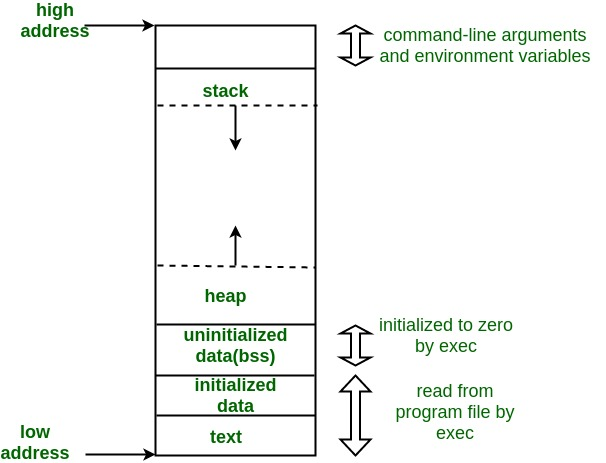
\includegraphics[totalheight=8cm]{images/Cmemory/memoryLayoutC.jpg}
	\begin{minipage}{.5\textwidth}
		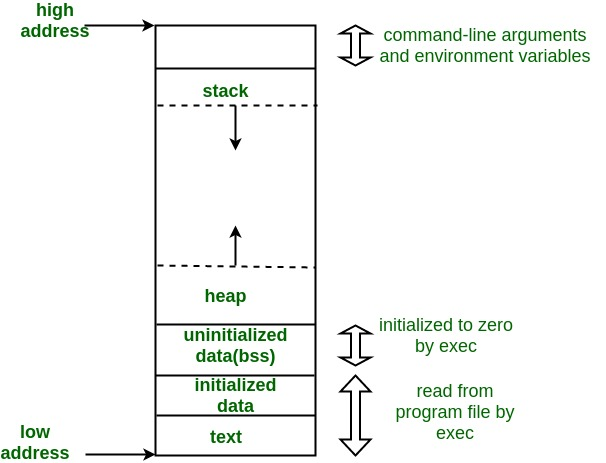
\includegraphics[width=1.2\textwidth]{images/Cmemory/memoryLayoutC.jpg}
		\caption{cf. \url{https://www.geeksforgeeks.org/memory-layout-of-c-program/}}
		\label{Fig:TypicalCMemoryLayout}
	\end{minipage}
\end{figure}

\subsection{Stack}


cf. \url{https://www.geeksforgeeks.org/memory-layout-of-c-program/}

Traditionally, stack area adjoined heap area and they grow in opposite direction. \\
When stack ptr meets heap ptr, free memory exhausted. \\
(with modern large address spaces, virtual memory techniques, they may be placed almost anywhere, but they still typically grow opposite direction)  \\

stack area contains program stack, UFO structure, typically located in higher parts of memory. \\
On standard x86, grows toward address 0. \\
"stack ptr" register tracks top of stack, adjusted to point to top each time a value is "pushed" onto stack. \\
set of values pushed for 1 function call is "stack frame", stack frame consists at minimum of return address. 

Newly called function allocates room on stack for its automatic and temporary variables. \\
$\Longrightarrow$ recursion: each time recursive function calls itself, new stack frame is used, so 1 set of variables (in recursion) doesn't interfere with variables from another instance of the function. 

cf. \href{https://www.tutorialspoint.com/where-are-static-variables-stored-in-c-cplusplus}{Where are static variables in C/C++? Tutorialspoint}

static variables remain in memory; lifetime is entire program, stored in data segment of memory (near heap); data segment is part of virtual address space of a program.

asked here \url{https://www.codingame.com/work/cpp-interview-questions/}, what is a static variable



cf. Ferres (2010) \cite{Ferr2010}

Stack and functions: When a function executes, it may add some of its state data to top of the stack (EY : 20171111, stack grows downward, so "top" is smallest address?); when function exits, stack is responsible for removing that data from stack.  

In most modern computer systems, each thread has a reserved region of memory, stack.  Thread's stack is used to store location of function calls in order to allow return statements to return to the correct location.  

\begin{itemize}
	\item OS allocates stack for each system-level thread when thread is created.  
	\item Stack is attached to thread, so when thread exits, that stack is reclaimed, vs. heap typically allocated by application at runtime, and is reclaimed when application exits.  
	\item When thread is created, stack size is set.  
	\item Each byte in stack tends to be reused frequently, meaning it tends to be mapped to the processor's cache, making if very fast.  
	\item Stored in computer RAM, \emph{just like} the heap.  
	\item Implemented with an actual stack data structure.  
	\item stores local data, return addresses, used for parameter passing  
	\item Stack overflow, when too much stack is used (mostly from infinite (or too much) recursion, and very large allocation)
	\item Data created on stack can be used without pointers.  
\end{itemize}

Also note, for \textbf{physical location in memory}, because of \href{http://en.wikipedia.org/wiki/Virtual_memory}{Virtual Memory}, makes your program think that you have access to certain addresses where physical data is somewhere else (even on hard disc!).  Addresses you get for stack are in increasing order as your call tree gets deeper.  

\href{http://stackoverflow.com/questions/79923/what-and-where-are-the-stack-and-heap/79988#79988}{memory management - What and where are the stack and heap? Stack Overflow, Tom Leys' answer}

\subsection{Stack overflow}  

If you use heap memory, and you overstep the bounds of your allocated block, you have a decent chance of triggering a segmentation fault (not 100%, since your block may be incidentally contiguous with another that you have previously allocated), says Ferres (2010) \cite{Ferr2010}.  

On stack, since variables created on stack are always contiguous with each other; writing out of bounds can change the value of another variable.  e.g. buffer overflow.  


\subsection{Heap}  

Heap contains a linked list of used and free blocks.  New allocations on the heap (by \verb|new| or \verb|malloc|) are satisfied by creating suitable blocks from free blocks.  

This requires updating list of blocks on the heap.  This meta information about the blocks on the heap is stored \emph{on the heap} often in a small area in front of every block.  

\begin{itemize}
	\item Heap size set on application startup, but can grow as space is needed (allocator requests more memory from OS)
	\item heap, stored in computer RAM, like stack.
\end{itemize}

\subsubsection{Memory leaks}  

Memory leaks occurs when computer program consumes memory, but memory isn't released back to operating system.  

"Typically, a memory leak occurs because dynamically allocated memory becomes unreachable."  (Ferres (2010) \cite{Ferr2010}).  

Programs \verb|./Cmemory/heapstack/Memleak.c| deliberately leaks memory by losing the pointer to allocated memory.  

Note, generally, the OS delays real memory allocation until something is written into it, so program ends when virtual addresses run out of bounds (per process limits).  

\subsection{More Segmentation Faults}  

The operating system (OS) is running the program (its instructions).  Only from the hardware, with \href{https://en.wikipedia.org/wiki/Memory_protection}{memory protection}, with the OS be signaled to a memory access violation, such as writing to read-only memory or writing outside of allotted-to-the-program memory, i.e. data segments.  On \verb|x86_64| computers, this \href{https://en.wikipedia.org/wiki/General_protection_fault}{general protection fault} is initiated by protection mechanisms from the hardware (processor).  From there, OS can signal the fault to the (running) process, and stop it (abnormal termination) and sometimes core dump. 

For \href{https://en.wikipedia.org/wiki/Virtual_memory}{virtual memory}, the memory addresses are mapped by program called \emph{virtual addresses} into \emph{physical addresses} and the OS manages virtual addresses space, hardcare in the CPU called memory management unit (\emph{MMU}) translates virtual addresses to physical addresses, and kernel manages memory hierarchy (eliminating possible overlays).  In this case, it's the \emph{hardware} that detects an attempt to refer to a non-existent segment, or location outside the bounds of a segment, or to refer to location not allowed by permissions for that segment (e.g. write on read-only memory).   

\subsubsection{Dereferencing a ptr to a NULL ptr (in C) at OS, hardware level}


The problem, whether it's for dereferencing a pointer that is a null pointer, or uninitialized pointer, appears to (see the \verb|./Cmemory/| subfolder) be at this instruction at the register level:  

\begin{lstlisting}
x000000000040056c <+38>:	movzbl (%rax),%eax

// or 

0x00000000004004be <+24>:	movss  %xmm0,(%rax)  
\end{lstlisting}

involving the register RAX, a temporary register and to return a value, upon assignment.  And in either case, register RAX has trying to access virtual (memory) address \verb|0x0| (to find this out in \verb|gdb|, do \verb|i r| or \verb|info register|).  

Modern OS's run user-level code in a mode, such as \emph{protected mode}, that uses "paging" (using secondary memory source than main memory) to convert virtual addresses into physical addresses.  

For each process (thread?), the OS keeps a \emph{page table} dictating how addresses are mapped.  Page table is stored in memory (and protected, so user-level code can't modify it).  For every memory access, given (memory) address, CPU translates address according to the page table.  

When address translation fails, as in the case that \emph{not all addresses are valid}, and so if a memory access generates an invalid address, the processor (hardware!) raises a \emph{page fault exception}.  "This triggers a transition from \emph{user mode} (aka \emph{current privilege level (CPL) 3} on x86/x86-64) into \emph{kernel mode} (aka CPL 0) to a specific location in the kernel's code, as defined by the \emph{interrupt descriptor table} (IDT)."  cf. [What happens in OS when we dereference a NULL pointer in C?](https://stackoverflow.com/questions/12645647/what-happens-in-os-when-we-dereference-a-null-pointer-in-c)


Kernel regains control and send signal (EY : 20171115 to the OS, I believe).   

In modern OS's, page tables are usually set up to make the address 0 an invalid virtual address.  

cf. [What happens in OS when we dereference a NULL pointer in C?](https://stackoverflow.com/questions/12645647/what-happens-in-os-when-we-dereference-a-null-pointer-in-c)

\part{C++}  

\section{Free Store}  


\href{http://www.gotw.ca/gotw/009.htm}{GotW \#9, Memory Management - Part I}



cf. 11.2 Introduction of Ch. 11 Select Operations \cite{Stro2013}.  




\section{Copy vs. Move}  
cf. 17.1 Introduction of Ch. 17 Construction, Cleanup, Copy, and Move of Stroustrup \cite{Stro2013}.  

Difference between \emph{move} and \emph{copy}: after a copy, 2 objects must have same value; whereas after a move, the source of the move isn't required to have its original value.  So moves can be used when source object won't be used again.  

Refs.: Sec. 3.2.1.2, Sec. 5.2, notion of moving a resource, Sec. 13.2-Sec.13.3, object lifetime and errors explored further in Stroustrup \cite{Stro2013}  


5 situations in which an object is copied or moved:   
\begin{itemize}
	\item as source of an \emph{assignment}
	\item as object initializer 
	\item as function argument
	\item as function return value
	\item as an exception  
\end{itemize}

\subsection{Copy constructor}

cf. \href{http://en.cppreference.com/w/cpp/language/copy_constructor}{Copy constructors, cppreference.com}

Copy constructor of class T is non-template constructor whose 1st parameter is \verb|T&, const T&, volatile T&|, or \verb|const volatile T&|.  

\subsubsection{Syntax}  

\begin{lstlisting}
class_name ( const class_name & )  
class_name ( const class_name & ) = default;  
class_name ( const class_name & ) = delete;
\end{lstlisting}  

\subsubsection{Explanation}  
\begin{enumerate}
	\item Typical declaration of a copy constructor.  
	\item Forcing copy constructor to be generated by the compiler.  
	\item Avoiding implicit generation of copy constructor.  
\end{enumerate}


Copy constructor called whenever an object is \textbf{initialized} (by \textbf{direct-initialization} or \textbf{copy-initialization}) from another object of same type (unless \textbf{overload resolution} selects better match or call is \textbf{elided} (???)), which includes  
\begin{itemize}
	\item initialization \verb|T a = b;| or \verb|T a(b);|, where b is of type T;  
	\item function argument passing: \verb|f(a);|, where a is of type T and f is \verb|void f(T t)|;  
	\item function return: \verb|return a;| inside function such as \verb|T f()|, where a is of type T, which has no \textbf{move constructor}.   
\end{itemize}

\subsubsection{Example}  
	
	\begin{lstlisting}
	struct A
	{
	int n;
	A(int n = 1) : n(n) { }
	A(const A& a) : n(a.n) { } // user-defined copy ctor
	};
	
	struct B : A
	{
	// implicit default ctor B::B()
	// implicit copy ctor B::B(const B&)
	};
	
	int main()
	{
	A a1(7);
	A a2(a1); // calls the copy ctor
	B b;
	B b2 = b;
	A a3 = b; // conversion to A& and copy ctor  
	}
	\end{lstlisting}  

i.e. cf. \href{http://www.geeksforgeeks.org/copy-constructor-in-cpp/}{Copy Constructor in C++}

\begin{definition}
	\textbf{Copy constructor} is a member function which initializes an object using another object of the same class.  
\end{definition}

\subsubsection{When is copy constructor called? } 
\begin{enumerate}
	\item When object of class returned by value 
	\item When object of class is passed (to a function) by value as an \textbf{argument}.  
	\item When object is constructed based on another object of same class  (or overloaded)  
	\item When compiler generates temporary object  
\end{enumerate}


However, it's not guaranteed copy constructor will be called in all cases, because C++ standard allows compiler to optimize the copy away in certain cases.  

\subsubsection{When is used defined copy constructor needed?  shallow copy, deep copy}  

If we don't define our own copy constructor, C++ compiler creates default copy constructor which does member-wise copy between objects.  

We need to define our own copy constructor only if an object has pointers or any run-time allocation of resource like file handle, network connection, etc.  

\subsubsection{Default constructor does only shallow copy.}  

\subsubsection{Deep copy is possible only with user-defined copy constructor.}  

We thus make sure pointers (or references) of copied object point to new memory locations.  

\subsubsection{Copy constructor vs. Assignment Operator}  

\begin{lstlisting}  
MyClass t1, t2; 
MyClass t3 = t1; 	// ----> (1)
t2 = t1; 			// -----> (2)
\end{lstlisting}

Copy constructor called when new object created from an existing object, as copy of existing object, in (1).  
Assignment operator called when already initialized object is assigned a new value from another existing object, as assignment operator is called in (2).  

\subsubsection{Why argument to a copy constructor should be const?  } 

cf. \href{http://www.geeksforgeeks.org/copy-constructor-argument-const/}{Why copy constructor argument should be const in C++?, geeksforgeeks.org}

\begin{enumerate}
	\item Use \verb|const| in C++ whenever possible so objects aren't accidentally modified.  
	\item e.g.  
\end{enumerate}

\begin{lstlisting}  
#include <iostream>  

class Test
{
/* Class data members */
public:
Test(Test &t) 	{ /* Copy data members from t */ } 
Test()			{ /* Initialize data members */ }
};

Test fun() 
{
Test t;
return t;
};

int main()
{
Test t1;
Test t2 = fun();  error: invalid initialization of non-const reference of type Test& from an rvalue of type Test
}
\end{lstlisting}

\verb|fun()| returns by value, so compiler creates temporary object which is copied to t2 using copy constructor (because this temporary object is passed as argument to copy constructor since compiler generates temp. object).  
Compiler error is because \textbf{compiler-created temporary objects cannot be bound to non-const references}. 



\subsection{Move Constructor}  

For a class, to control what happens when we move, or move and assign object of this class type, use special member function \emph{move constructor}, \emph{move-assignment operator}, and define these operations.  Move constructor and move-assignment operator take a (usually nonconst) rvalue reference, to its type.  Typically, move constructor moves data from its parameter into the newly created object.  After move, it must be safe to run the destructor on the given argument.  cf. Ch. 13 of Lippman, Lajole, and Moo (2012) \cite{LLM2012}



\section{vtable; virtual table}  

I was given this answer to a question I posed to a 20 year C++ veteran and it was such an important answer (as I did not know a virtual table existed, at all before), that I will copy this, repeat this and explore this extensively:  

"The keyword you're looking for is virtual table: " \href{https://stackoverflow.com/questions/99297/how-are-virtual-functions-and-vtable-implemented}{How are virtual functions and vtable implemented?, stackoverflow}  

Original question, from \href{https://stackoverflow.com/users/3153/brian-r-bondy}{Brian R. Bondy}:  

\subsection{How are virtual functions and vtable implemented?}

We all know what virtual functions are in C++, but how are they implemented at a deep level?

Can the vtable be modified or even directly accessed at runtime?

Does the vtable exist for all classes, or only those that have at least one virtual function?

Do abstract classes simply have a NULL for the function pointer of at least one entry?

Does having a single virtual function slow down the whole class? Or only the call to the function that is virtual? And does the speed get affected if the virtual function is actually overwritten or not, or does this have no effect so long as it is virtual.

Answer from \emph{community wiki}:  

\subsubsection{How are virtual functions implemented at a deep level?}

From \href{http://wayback.archive.org/web/20100209040010/http://www.codersource.net/published/view/325/virtual_functions_in.aspx}{"Virtual Functions in C++"}

Whenever a program has a virtual function declared, a v-table is constructed for the class. The v-table consists of addresses to the virtual functions for classes that contain one or more virtual functions. The object of the class containing the virtual function contains a virtual pointer that points to the base address of the virtual table in memory.   

Whenever there is a virtual function call, the v-table is used to resolve to the function address. 

An object of the class that contains one or more virtual functions contains a virtual pointer called the vptr at the very beginning of the object in the memory. Hence the size of the object in this case increases by the size of the pointer. This vptr contains the base address of the virtual table in memory.  

Note that virtual tables are class specific, i.e., there is only one virtual table for a class irrespective of the number of virtual functions it contains. This virtual table in turn contains the base addresses of one or more virtual functions of the class. At the time when a virtual function is called on an object, the vptr of that object provides the base address of the virtual table for that class in memory. This table is used to resolve the function call as it contains the addresses of all the virtual functions of that class. This is how dynamic binding is resolved during a virtual function call.

cf. \href{http://wayback.archive.org/web/20100209040010/http://www.codersource.net/published/view/325/virtual_functions_in.aspx}{"Virtual Functions in C++"}

\subsubsection{What is a Virtual Function?}  

A virtual function is a member function of a class, whose functionality can be over-ridden in its derived classes. It is one that is declared as virtual in the base class using the virtual keyword. The virtual nature is inherited in the subsequent derived classes and the virtual keyword need not be re-stated there. The whole function body can be replaced with a new set of implementation in the derived class. 

\subsubsection{What is Binding?}  

Binding is associating an object or a class with its member.   If we call a method \verb|fn()| on an object \verb|o| of a class \verb|c|, we say that object \verb|o| is binded with method \verb|fn()|.  

This happens at \emph{compile time} and is known as \emph{static} - or \emph{compile-time} binding.   
Calls to virtual member functions are resolved during \emph{run-time}.  This mechanisms is known as \emph{dynamic-binding.}   

The most prominent reason why a virtual function will be used is to have a different functionality in the derived class.  The difference between a non-virtual member function and a virtual member function is, the non-virtual member functions are resolved at compile time.  


\subsubsection{How does a Virtual Function work?}  

When a program (code text?) has a virtual function declared, a \textbf{v-table} is \emph{constructed} for the class.  

The v-table consists of addresses to virtual functions for classes that contain 1 or more virtual functions.  \\
The object of the class containing the virtual function \emph{contains a virtual pointer} that points to the base address of the virtual table in memory.  An object of the class that contains 1 or more virtual functions contains a virtual pointer called the \textbf{vptr} at the very beginning of the object in the memory.  (Hence size of the object in this case increases by the size of the pointer; "memory/size overhead.")  \\

This vptr is added as a hidden member of this object.  As such, compiler must generate "hidden" code in the \textbf{constructors} of each class to initialize a new object's vptr to the address of its class's vtable.  


Whenever there's a virtual function call, vtable is used to resolve to the function address.  
This vptr contains base address of the virtual table in memory.  \\

Note that virtual tables are class specific, i.e. there's only 1 virtual table for a class, irrespective of number of virtual functions it contains, i.e.  

vtable is same for all objects belonging to the same class, and typically is shared between them.    
  

This virtual table in turn contains base addresses of 1 or more virtual functions of the class.  

At the time when a virtual function is called on an object, the vptr of that object provides the base address of the virtual table for that class in memory.  This table is used to resolve the function call as it contains the addresses of all the virtual functions of that class.  This is how dynamic binding is resolved during a virtual function call, i.e.  

class (inherited or base/parent) cannot, generally, be determined \emph{statically} (i.e. \textbf{compile-time}), so compiler can't decide which function to call at that (compile) time.  (Virtual function) call must be dispatched to the right function \emph{dynamically} (i.e. \textbf{run-time}).  



\subsubsection{Virtual Constructors and Destructors}  

A constructor cannot be virtual because at the time when constructor is invoked, the vtable wouldn't be available in memory.  Hence, we can't have a virtual constructor.  

A virtual destructor is 1 that's declared as virtual in the base class, and is used to ensure that destructors are called in the proper order.  Remember that destructors are called in reverse order of inheritance.  If a base class pointer points to a derived class object, and we some time later use the delete operator to delete the object, then the derived class destructor is not called.  

Finally, the article \href{http://wayback.archive.org/web/20100209040010/http://www.codersource.net/published/view/325/virtual_functions_in.aspx}{"Virtual Functions in C++"} concludes, saying, "Virtual methods should be used judiciously as they are slow due to the overhead involved in searching the virtual table. They also increase the size of an object of a class by the size of a pointer. The size of a pointer depends on the size of an integer."  I will have to check this with other references, because, first of all, how then would class inheritance be otherwise implemented?  

cf. \href{https://stackoverflow.com/questions/99297/how-are-virtual-functions-and-vtable-implemented}{How are virtual functions and vtable implemented?, stackoverflow}  

\subsubsection{Can the vtable be modified or even directly accessed at runtime?  No.}  

"Universally, I believe the answer is "no". You could do some memory mangling to find the vtable but you still wouldn't know what the function signature looks like to call it. Anything that you would want to achieve with this ability (that the language supports) should be possible without access to the vtable directly or modifying it at runtime. Also note, the C++ language spec does not specify that vtables are required - however that is how most compilers implement virtual functions."  

\subsubsection{Do abstract classes simply have a NULL for the function pointer of at least one entry?  Some do place NULL pointer in vtable, some place pointer to dummy method; in general, undefined behavior}

The answer is it is unspecified by the language spec so it depends on the implementation. Calling the pure virtual function results in undefined behavior if it is not defined (which it usually isn't) (ISO/IEC 14882:2003 10.4-2). In practice it does allocate a slot in the vtable for the function but does not assign an address to it. This leaves the vtable incomplete which requires the derived classes to implement the function and complete the vtable. Some implementations do simply place a NULL pointer in the vtable entry; other implementations place a pointer to a dummy method that does something similar to an assertion.

Note that an abstract class can define an implementation for a pure virtual function, but that function can only be called with a qualified-id syntax (ie., fully specifying the class in the method name, similar to calling a base class method from a derived class). This is done to provide an easy to use default implementation, while still requiring that a derived class provide an override.

\subsubsection{Does having a single virtual function slow down the whole class or only the call to the function that is virtual?  No, but space overhead is there}  

"This is getting to the edge of my knowledge, so someone please help me out here if I'm wrong!

I believe that only the functions that are virtual in the class experience the time performance hit related to calling a virtual function vs. a non-virtual function. The space overhead for the class is there either way. Note that if there is a vtable, there is only 1 per class, not one per object."

\subsubsection{Does the speed get affected if the virtual function is actually overridden or not, or does this have no effect so long as it is virtual?  No, but space overhead is there}  

"I don't believe the execution time of a virtual function that is overridden decreases compared to calling the base virtual function. However, there is an additional space overhead for the class associated with defining another vtable for the derived class vs the base class."  

\subsection{pImpl, shallow copy, deep copy}  

cf. Item 22: "When using the Pimpl Idiom, define special member functions in the implementation file," pp. 147 of Meyers (2014) \cite{ScMe2014}.  

\begin{lstlisting}
class Widget { 			// still in header "widget.h" 
public:
Widget();
~Widget();		// dtor is needed-see below 
... 

private:
struct Impl;	// declare implementation struct 
Impl *pImpl;	// and pointer to it
};
\end{lstlisting}

Because \verb|Widget| no longer mentions types \verb|std::string, std::vector|, and \verb|Gadget, Widget| clients no longer need to \verb|\#include| headers for these types.  That speeds compilation.  

\emph{incomplete type} is a type that has been declared, but not defined, e.g. \verb|Widget::Impl|.  There are very few things you can do with an incomplete type, but declaring a pointer to it is 1 of them.  

\verb|std::unique_ptr|s is advertised as supporting incomplete types.  But, when \verb|Widget w;|, \verb|w|, is destroyed (e.g. goes out of scope), destructor is called and if in class definition using \verb|std::unique_ptr|, we didn't declare destructor, compiler generates destructor, and so compiler inserts code to call destructor for \verb|Widget|'s data member \verb|m_Impl| (or \verb|pImpl|).  

\verb|m_Impl| (or \verb|pImpl|) is a \verb|std::unique_ptr<Widget::Impl>|, i.e., a \verb|std::unique_ptr| using default deleter. The default deleter is a function that uses \verb|delete| on raw pointer inside the \verb|std::unique_ptr|.  Prior to using \verb|delete|, however, implementations typically have default deleter employ C++11's \verb|static_assert| to ensure that raw pointer doesn't point to an incomplete type.  When compiler generates code for the destruction of the \verb|Widget w|, then, it generally encounters a \verb|static_assert| that fails, and that's usually what leads to the error message.  

To fix the problem, you need to make sure that at point where code to destroy \verb|std::unique_ptr<Widget::Impl>| is generated, \verb|Widget::Impl| is a complete type.  The type becomes complete when its definition has been seen, and \verb|Widget::Impl| is defined inside \verb|widget.cpp|.  For successful compilation, have compiler see body of \verb|Widget|'s destructor (i.e. place where compiler will generate code to destroy the \verb|std::unique_ptr| data member) only inside \verb|widget.cpp| after \verb|Widget::Impl| has been defined.  

For compiler-generated move assignment operator, move assignment operator needs to destroy object pointed to by \verb|m_Impl| (or \verb|pImpl|) before reassigning it, but in the \verb|Widget| header file, \verb|m_Impl| (or \verb|pImpl|) points to an incomplete type.  Situation is different for move constructor.  Problem there is that compilers typically generate code to destroy \verb|pImpl| in the event that an exception arises inside the move constructor, and destroying \verb|pImpl| requires \verb|Impl| be complete.  

Because problem is same as before, so is the fix - \emph{move definition of move operations into the implementation file}.  

For copying data members, support copy operations by writing these functions ourselves, because (1) compilers won't generate copy operations for classes with move-only types like \verb|std::unique_ptr| and (2) even if they did, generated functions would copy only the \verb|std::unique_ptr| (i.e. perform a \emph{shallow copy}), and we want to copy what the pointer points to (i.e., perform a \emph{deep copy}).  

If we use \verb|std::shared_ptr|, there'd be no need to declare destructor in \verb|Widget|.  

Difference stems from differing ways smart pointers support custom deleters.  For \verb|std::unique_ptr|, type of deleter is part of type of smart pointer, and this makes it possible for compilers to generate smaller runtime data structures and faster runtime code.  A consequence of this greater efficiency is that pointed-to types must be complete when compiler-generated special functions (e.g. destructors or move operations) are used.  For \verb|std::shared_ptr|, type of deleter is not part of the type of smart pointer.  This necessitates larger runtime data structures and somewhat slower code, but pointed-to types need not be complete when compiler-generated special functions are employed.  

\part{Integers, numeric encodings, number representation, binary representation, hexidecimal representation}

\section{Introduction:} 
\texttt{int} $\neq \mathbb{Z}$, \texttt{float} $\neq \mathbb{R}$

cf. \href{https://www.cs.utexas.edu/users/fussell/courses/cs429h/lectures/Lecture_1-429h.pdf}{Systems 1, Introduction to Computer Systems, Introduction lecture at University of Texas, CS429; Don Fussell}.

\texttt{int} $\neq \mathbb{Z}$, \texttt{float} $\neq \mathbb{R}$

e.g. $x^2 \geq 0$? 

\texttt{float}: Yes!  \\
\texttt{int}: $40000 \times 40000 \to 1600000000$ \\
\phantom{int} $50000 \times 50000 \to $ ??

Is $(x+y) + z = x + (y +z)?$

\texttt{unsigned} and \texttt{signed int}: Yes!

\texttt{float}'s 
\[
\begin{gathered}
(1e20 + -1e20) + 3.14 \to 3.14 \\
1e20 + (-1e20 + 3.14) \to ??
\end{gathered}
\]

Can't assume "usual" properties due to finiteness of representations, so that integer operations satisfy "ring" properties
- commutativity, associativity, distributivity

floating point operations satisfy "ordering" properties
- monotonicity, values of signs


\section{Bits and Bytes}

cf. \href{https://www.cs.utexas.edu/users/fussell/courses/cs429h/lectures/Lecture_2-429h.pdf}{Lecture 2, Bits and Bytes, CS429}.

Consider a (number) system with radix or base $b$ ($b>1$), \\
string of digits $d_1, \dots , d_n$, \\
\begin{equation}
c = \sum_{i=1}^n d_i b^{n-i}, \qquad \, 0 \leq d_i < b \qquad \forall \, i = 1 \dots n 
\end{equation}

with notation $c \equiv c_b$ to help denote the base or "radix", e.g. $15213_{10}$, $00000000_2$.

Byte $\equiv B$, 1 Byte $ = 8$ bits. Note that $2^8 = 256$

e.g. Binary $00000000_2$ to $11111111_2$ \\
Decimal: $0_{10}$ to $255_{10}$ \\
Hexadecimal: $00_{16}$ to $FF_{16}$

\subsection{Machine Words}

Machine has "Word size".

Nominal size of integer-valued data, including addresses.

\subsection{Word-oriented Memory Organization}

Addresses specify Byte locations. 

Addresses of successive words differ by 4 (32-bit) or 8 (64-bit).

32-bit words:

Addr = 0000, Addr = 0004

64-bit words:

Addr = 0000, Addr = 0008

\subsection{Byte-ordering: Big-Endian, Little-Endian}

$b = 8$

\begin{equation}
c = \sum_{i=0}^{n-1} d_i 8^{n-1 -i}
\end{equation}

\textbf{Big-Endian}: Least significant byte has highest address.

For address $a$, 
\[
\begin{gathered}
a \mapsto d_0 \\
a+1 \mapsto d_1 \\
\vdots \\
a+n-1 \mapsto d_{n-1}
\end{gathered}
\]

\textbf{Little-Endian}: Least significant byte has lowest address
\[
\begin{gathered}
a \mapsto d_{n-1}  \\
a+1 \mapsto d_{n-2} \\
\vdots \\
a+n -1 \mapsto d_0
\end{gathered}
\]

\subsection{Representing Strings}

C Strings

- represented by array of characters, each character encoded in ASCII format 
- string should by null-terminated meaning final character $=0$

\subsection{Machine-Level Code Representation}

Encode program as sequence of Instructions. 

Each simple operation
- arithmetic operation, read or write memory, conditional branch.
- instructions encoded as bytes, 
i.e. programs are byte sequences too!

\subsection{Boolean Algebra}

Boole's Algebraic representation of logic.

And: \\
$A \& B = 1$ when both $A=1$ and $B=1$

Or: \\
$A | B = 1$ when either $A=1$ or $B=1$

Not: \\
${}^{\sim}A= 1$ when $A=0$, \\
${}^{\sim}A= 0$ when $A=1$, \\

Exclusive-Or (Xor)
$A {}^{\wedge} B = 1$ when either $A=1$ or $B=1$, but not both

\begin{center}
	\begin{tabular}{ l | c  c }
		${}^{\wedge}$ & 0 & 1 \\ \hline 
		0 & 0 & 1 \\
		1 & 1 & 0
	\end{tabular}
\end{center}

\subsubsection{Application of Boolean Algebra}

Claude Shannon 1937 MIT Master's Thesis. Encode closed switch as 1, open switch as 0. Connection when $A\& \sim B | \sim A \& B = A \wedge B$

\subsubsection{Integer Algebra}

$\langle \mathbb{Z}, +, *, - , 0 , 1 \rangle$ forms a ring

\subsubsection{Boolean Algebra}

$\langle \lbrace 0, 1 \rbrace , |, \& , \sim, 0, 1 \rangle $ forms a "Boolean algebra"

Or ($|$) is "sum" operation. \\
And ($\&$) is "product" operation. \\
$\sim$ is "complement" operation. \\
$0$ is additive identity. \\
$1$ is multiplicative identity.

cf. \url{https://en.wikipedia.org/wiki/Bitwise_operation}

Bitwise OR may be used to set to 1 selected bits of register. e.g. fourth bit of 0010 may be set by performing bitwise OR with pattern with only 4th bit set.

Bitwise AND is equivalent to multiplying corresponding bits. Thus, if both bits in compared position are 1, bit in resulting binary representation is ($1 \times 1 = 1$); otherwise result is 0 ($1 \times 0 = 0$ and $0 \times 0 = 0$).

Operation may be used to determine whether particular bit is set (1) or clear (0). e.g. given bit pattern 0011 (decimal 3), to determine whether 2nd bit is set, use bitwise AND with bit pattern containing 1 only in 2nd. bit. Because result 0010 is non-zero, we know 2nd. bit in original pattern is set. This is often called \emph{bit masking} (by analogy, use of masking tape covers, or \emph{masks}, portions that are not of interest)

Bitwise AND may be used to clear selected bits (or flags) of a register in which each bit represents an individual Boolean state.
\begin{itemize}
	\item This technique is an efficient way to store a number of Boolean values using as little memory as possible.
	\item Also, easy to check parity (even or odd?) of binary number by checking value of lowest valued bit.
\end{itemize}

Bitwise XOR may be used to invert selected bits in a register (also called toggle or flip). Any bit may be toggled by XORing with 1. e.g. given bit pattern 0010, 2nd and 4th bits may be toggled by bitwise XOR with bit pattern containing 1 in 2nd. and 4th. positions.


Consider Boolean Ring:
\[
\langle \lbrace 0 , 1 \rbrace, \wedge, \&, I, 0 , 1 \rangle \simeq \mathbb{Z}_2 \equiv  \text{ integers} \mod{2} 
\]
where $I$ is identity operation $I(A) = A$, \\
and 
$A\wedge A = 0$ is the additive inverse (existence) property.

\subsubsection{De Morgan's Laws}

\[
\begin{gathered}
A \& B = \sim (\sim A | \sim B) \\
A | B = \sim (\sim A \& \sim B)
\end{gathered}
\]

\subsubsection{Exclusive-Or using Inclusive Or}

\[
\begin{gathered} 
A \wedge B = (\sim A \& B) | (A \& \sim B) \\
A \wedge B = (A | B) \& \sim (A \& B)
\end{gathered} 
\]

All properties of Boolean Algebra apply to bit vectors.

\subsection{Representing and Manipulating Sets; bit vectors as sets}

Width $w$ bit vector represents subsets of $\lbrace 0 ,\dots, w-1 \rbrace$, s.t. for $a\in \lbrace 0 ,1 \rbrace^w$, $a_j \in \lbrace 0 , 1 \rbrace$, $\forall \, j = 0,1,\dots w -1$. 

\qquad \\
If $a_j = 1, j \in A$; otherwise, \\
If $a_j =0$, $j \notin A$
\qquad \\

\subsubsection{Operations}

\qquad \\
$\& \to $ intersection \\
$| \to $ union \\
$\wedge \to $ symmetric difference \\
$\sim \to $ complement
\qquad \\

Logic operations in C: $\& \&$, $||$, $!$ 

Shift operations

cf. \href{https://www.cs.utexas.edu/users/fussell/courses/cs429h/lectures/Lecture_3-429h.pdf}{Systems 1, Integers lecture at University of Texas, CS429} is a \textbf{very good lecture}; both \emph{mathematically rigorous} and full of useful, \emph{clear} examples.

\section{Unsigned integers}

Consider $\mathbb{Z}^+_{2^w} \to \mathbb{Z}^+$, where $\mathbb{Z}^+_{2^w}$ represent "unsigned" integers. 
\begin{equation}
\begin{gathered}
\mathbb{Z}^+_{2^w} \to \mathbb{Z}^+ \\ 
(x_0, x_1 , \dots , x_{w-1}) \mapsto \sum_{i=0}^{w-1} x_i \cdot 2^i 
\end{gathered}
\end{equation}

To recap using CS429's notation, for an unsigned integer $x$, \\
$B2U \equiv $ base-2-unsigned \\
\[
B2U(x) = \sum_{i=0}^{w-1} x_i \cdot 2^i 
\]
where $B2U : "\mathbb{Z}^+" \to \mathbb{Z}^+_{2^w}$

So $w$ is the total number of "bits" to represent $x$.



For hexidecimal (-based) numbers, observe this relationship: 
\begin{equation}
2^w = 16^v = 2^{4v} \text{ so } w =4v
\end{equation}

So for a hexidecimal number, $v$ hexidecimal numbers represent $w=4v$ bits. 

Observe that 
\begin{equation}
\mathbb{Z}^+_{2^w} = \lbrace 0 , \dots 2^w - 1 \rbrace 
\end{equation}

Also, \textbf{modular addition} $(\mathbb{Z}^+_{2^w}, +)$ forms an \textbf{abelian group}.

\section{Two's complement}

cf. \href{https://www.cs.utexas.edu/users/fussell/courses/cs429h/lectures/Lecture_3-429h.pdf}{Systems 1 Integers}

Denote the notation for so-called "two's complement" numbers as $\mathbb{Z}_{2^w}$, which is a representation for integers in such a manner:

\begin{equation}
\begin{gathered}
\mathbb{Z}_{2^w} \to \mathbb{Z} \\
%(x_0, x_1, \dots x_{w-1}) 
(x_{w-1}, x_{w-2}, \dots x_0) \mapsto -x_{w-1} \cdot 2^{w-1} + \sum_{i=0}^{w-2} x_i \cdot 2^i
\end{gathered}
\end{equation}
with
\begin{equation}
\mathbb{Z}_{2^w} = \lbrace - 2^{w-1} \dots 2^{w-1} -1 \rbrace
\end{equation}

To recap using CS429's notation, for integer $x \in \mathbb{Z}$, \\
$B2T \equiv $ base-2-Two's complement \\
\[
B2T(x) = -x_{w-1} \cdot 2^{w-1} + \sum_{i=0}^{w-2} x_i \cdot 2^i
\]
where $B2T: "\mathbb{Z}" \to \mathbb{Z}_{2^w} = \lbrace -2^{w-1} \dots 2^{w-1} - 1 \rbrace$


Observe that 
\begin{equation}
\begin{gathered}
\max{ \left( \mathbb{Z}^+_{2^w} \right) } = 2 \max{ \mathbb{Z}_{2^w} } + 1 \\
| \min{ \mathbb{Z}_{2^w} } | = \max{ \mathbb{Z}_{2^w} } + 1
\end{gathered}
\end{equation}

To recap and to clean up and unify the notation, recall the following: \\
radix (i.e. base) $b$ \\
string of digits $d_1, \dots d_n$, 
\[
c = \sum_{i=1}^n d_i b^{n-i} , \quad \, 0 \leq d_i < b \quad \, \forall \, i = 1 \dots n
\]
cf. \href{https://en.wikipedia.org/wiki/Radix}{wikipedia, "Radix"}
i.e.
\[
\begin{gathered}
\lbrace 0 ,1 ,\dots b-1 \rbrace^n \to \mathbb{Z} \\ 
(d_1, \dots d_n) \mapsto c = \sum_{i=1}^n d_i b^{n-i}
\end{gathered}
\]
or (alternative notation),
\[
\begin{gathered}
\lbrace 0 1, ,\dots b-1 \rbrace^w \to \mathbb{Z} \\ 
(d_{w-1}, d_{w-2}, \dots, d_0) \mapsto c = \sum_{i=0}^{w-1} d_i b^i 
\end{gathered}
\]

In Fussell's notation, Fussell (2011) \cite{Fuss2011},
\[
\begin{gathered}
\begin{gathered}
\lbrace 0 ,1, \dots b-1 \rbrace^w \to \mathbb{Z} \text{ or } \mathbb{Z}^+_{2^w} \to \mathbb{Z}^+ \\
(x_{w-1}, x_{w-2}, \dots x_0) \mapsto c = \sum_{i=0}^{w-1} x_i 2^i, \, x_i < 2
\end{gathered} \\
B2U(X) = B2U(x_{w-1}, \dots x_0) = \sum_{i=0}^{w-1} x_i 2^i
\end{gathered}
\]
I will also use this notation:
\[
B2U(x_w, x_{w-1}, \dots x_1) = \sum_{i=1}^w x_i 2^{i-1}
\]

For the \emph{Two's Complement},

\[
\begin{gathered}
B2T(X) = B2T(-x_{w-1}, x_{w-2}, \dots x_0) = -x_{w-1}2^{w-1} + \sum_{i=0}^{w-2} x_i 2^i \\
\lbrace 0 , 1, \dots b-1 \rbrace^w \to \mathbb{Z} 
\end{gathered}
\]
or with the notation I'll use,
\[
B2T(-x_w, x_{w-1}, \dots x_1) = -x_w 2^{w-1} + \sum_{i=1}^{w-1} x_i 2^{i-1}
\]
Note that for hexadecimal,
\[
c = \sum_{i=1}^w x_i 2^{i-1} = \sum_{i=1}^v y_i (16)^{i-1} = \sum_{i=1}^v y_i 2^{4i-4}
\]
$v$ hexadecimal digits $\leftrightarrow  4v = w$ bits.

\subsection{Numeric Ranges}

For unsigned values, 
\[
\begin{gathered}
\begin{gathered} 
\text{UMin} = 0 \\
000 \dots 0 
\end{gathered} \\
\text{UMax} = 2^w - 1  
\end{gathered}
\]

For why UMax $=2^w -1$, consider the geometric progression:
\[
\begin{gathered}
\sum_{k=1}^n ar^{k-1} \\
(1-r) \sum_{k=1}^n ar^{k-1} = a-ar^n \text{ or } \sum_{k=1}^n ar^{k-1} = \frac{a(1-r^n) }{1-r} \\
\Longrightarrow \sum_{i=1}^w 2^{i-1} = \frac{1-2^w}{1-2} = 2^w - 1
\end{gathered}
\]

\[
\begin{gathered}
\begin{gathered} 
\text{TMin} = -2^{w-1} \\
100 \dots 0 
\end{gathered} \\
\begin{gathered} 
\text{TMax} = 2^{w-1} - 1
011\dots 1
\end{gathered}
\end{gathered} 
\]

$-1 \leftrightarrow 111 \dots 1$


\subsection{Negating with complement}

\begin{equation}
\begin{gathered}
\begin{gathered} 
\sim : \mathbb{Z}_{2^w} \to \mathbb{Z} \text{ s.t. } \\
\sim x + 1 = -x \quad \, \forall \, x \in \mathbb{Z}_{2^w} \\
\end{gathered}  \\
\begin{gathered} 
\sim : \mathbb{Z}^+_{2^w} \to \mathbb{Z} \text{ s.t. } \\
\sim x = 2^w- 1 -x 
\end{gathered}
\end{gathered}
\end{equation}

\subsection{Power of 2 Multiply with shift (left shift bitwise operation) }

For both $\mathbb{Z}^+_{2^w}$, $\mathbb{Z}_{2^w}$, 

\begin{equation}
u << k = u \cdot 2^k \qquad \, \forall \, u \in \mathbb{Z}^+_{2^w} \text{ or } \mathbb{Z}_{2^w} \text{and } k \in \mathbb{Z}
\end{equation}

\subsection{Unsigned power-of-2 Divide, with shift (right shift bitwise operator)}

\begin{equation}
u >> k = \lfloor u / 2^k \rfloor \qquad \, \forall \, u \in \mathbb{Z}^+_{2^w}, \quad \, k \in \mathbb{Z}  
\end{equation}

\section{Endianness} 

Consider \emph{address} $\in \mathbb{Z}^+_{2^3}$.  Consider a \emph{value} $\in \mathbb{Z}^+_{2^3}$ or $\mathbb{Z}_{2^3}$. 

$\forall \, (x_0, x_1, \dots x_{w-1}) \in \mathbb{Z}^+_{2^3} \text{ or } \mathbb{Z}_{2^3}$

Given address $a$, 

\subsection{Big-endian}

\begin{definition}[Big-endian]
	Most-significant byte value is at the lowest address, i.e. 
	\begin{equation}
	\begin{gathered}
	a \mapsto x_{w-1} \\
	a+1 \mapsto x_{w-2} \\ 
	a+2 \mapsto x_{w-3} \\ 
	\vdots \\
	a+w - 1 \mapsto x_0 
	\end{gathered}
	\end{equation}
\end{definition} 

\subsection{Little-endian}

\begin{definition}[Little-endian]
	Least-significant byte value is at the lowest address, i.e.
	\begin{equation}
	\begin{gathered}
	a \mapsto x_0 \\
	a + 1 \mapsto x_1 \\
	\vdots \\
	a+w - 1 \mapsto x_{w-1}
	\end{gathered}
	\end{equation}
	
	For Little-endian $\to \mathbb{Z}$, \\
	$( \text{ addresses } ) \in \mathbb{Z}^+_{2^3} \mapsto \mathbb{Z}$, \\
	$a \mapsto (x_0, x_1, \dots x_{w-1})$
	
	For $\mathbb{Z} \to $ Big-endian, \\
	$n \mapsto (x_{w-1}, x_{w-2}, \dots x_0)$.
	
	Instead, to tackle the confusing problem of byte ordering, think about the integer as itself first, and then consider \emph{mapping multibyte binary values to memory}.
	
	\begin{equation}
	\begin{gathered}
	\mathbb{Z} \to \left( \mathbb{Z}_{2^w} \longleftarrow \mathbb{Z}_{(2^3)^w} = \textbf{addresses}  \right) \\
	\begin{aligned}
	& \mathbb{Z} \ni (x_{w-1}, x_{w-2}, \dots x_1, x_0) \xmapsto{\text{Little-Endian}}  & \left((x_0, x_1 , \dots x_{w-2}, x_{w-1}) \longleftarrow\!\shortmid \,  (a, a+1, \dots a + w-2, a+w-1)\right) \\
	& \mathbb{Z} \ni (x_{w-1}, x_{w-2}, \dots x_1, x_0) \xmapsto{\text{Big-Endian}}  & \left((x_{w-1}, x_{w-2} , \dots x_{1}, x_{0}) \longleftarrow\!\shortmid \,  (a, a+1, \dots a + w-2, a+w-1)\right) 
	\end{aligned}
	\end{gathered}
	\end{equation}
	
\end{definition}

\part{Floating Point Numbers}

\section{Floating point, IEEE Floating}

IEEE Standard 754

Recall our previous notation for the sum representation of a number $c$:

\begin{equation}
c = \sum_{i=1}^n d_i b^{n-i}; \qquad \, 0 \leq d_i < b , \quad \forall \, i = 1\dots n 
\end{equation}
e.g.
\[
c = 42_{10} = 4 \cdot 10^{2-1} + 2\cdot 10^{2-2} = d_1 b^{n-1} + d_2 b^{n-2}
\]
By writing the exponent to be $n-i$, then we can write the digit representing the largest value in the summation "starting from the left" as such: \\
\[
c = (d_1, d_2, \dots d_{n-1}, d_n)
\]
e.g. $(4, 2) = 42$.

However, the \href{https://www.cs.utexas.edu/users/fussell/courses/cs429h/lectures/Lecture_4-429h.pdf}{CS429h} lectures uses the following notation for the \texttt{unsigned int}:

\[
B2U(X) = \sum_{i=0}^{w-1} x_i 2^i \text{ or } (x_{w-1}, x_{w-2}, \dots x_1, x_0) \mapsto \sum_{i=0}^{w-1} x_i 2^i
\]
e.g. $(x_3, x_2, x_1, x_0) = (1, 0, 1, 1) \mapsto x_0 2^0 + x_1 2^1 + x_2 2^2 + x_3 2^3$

\subsection{Fractional Binary Numbers}

\subsubsection{Representation}

Bits to right of "binary point" represent fractional powers of 2. \\
Binary number is used to represent a rational number, which in turn is a floating-point \emph{representation}. 
\begin{equation}
\sum_{k=-j}^i b_k \cdot 2^k \equiv \sum_{k=-M}^N b_k 2^k
\end{equation}
\begin{equation}
b \equiv (b_N, b_{N-1}, \dots b_1, b_0, b_{-1}, \dots b_{-M}) \mapsto \sum_{k=-M}^n b_k 2^k \equiv c
\end{equation}

i.e. 
\[
\sum_{k=-M}^N b_k 2^k = b_N \cdot 2^N + b_{N-1} 2^{N-1} + \dots + b_1 \cdot 2 + b_0 \cdot 1 + b_{-1} \cdot \frac{1}{2} + \dots + b_{-M} \cdot 2^{-M}
\]
e.g. $101.11_2 \mapsto 5 \frac{3}{4} $ 

Divide by 2 by shifting right: 
\begin{equation}
\begin{gathered} 
\frac{c}{2} = \sum_{k=-M}^N b_k 2^k/2 = \sum_{k=-M-1}^{N-1} b_{k+1} 2^k \\	
(b_N, b_{N-1}, \dots b_{-M}) \xrightarrow{ \cdot \frac{1}{2}} (0, b_N, b_{N-1}, \dots b_{-M-1}, b_{-M})
\end{gathered} 
\end{equation}

Multiply by 2 by shifting left:

\begin{equation}
\begin{gathered}
2  \cdot c = \sum_{k=-M}^N b_k \cdot 2^k \cdot 2 = \sum_{k=-M+1}^{N+1} b_{k-1} 2^k \\
(b_N, b_{N-1}, \dots b_{-M}) \xrightarrow{ \cdot 2} (b_N, b_{N-1}, \dots b_{-M} , 0)
\end{gathered}
\end{equation}

This implies that we first choose the "most significant bit", the digit $b_k$ representing the largest value in the sum representation to start from the \emph{left}.

Numbers of form $0.111111\dots_2$ just below 1.0 (remember those are bits, 0 or 1).

\[
\frac{1}{2} + \frac{1}{4} + \frac{1}{8} + \dots + \frac{1}{2^{M}} + \dots \to 1.0
\]
Use $1.0 - \epsilon$ notation.

\subsubsection{Limitation of representable numbers}

Can only exactly represent numbers of form $\frac{x}{2^k}$

The other numbers have repeating bit representations.

\begin{center}
	\begin{tabular}{ l | l }
		\hline
		Value & Representation \\ \hline
		$\frac{1}{3}$ & $0.0101010101[01]\dots_2$ \\ 
		$\frac{1}{5}$ & $0.001100110011[0011] \dots 2$ \\
		$\frac{1}{10}$ & $0.0001100110011[0011] \dots_2$ \\
		\hline
	\end{tabular}
\end{center}

\subsubsection{Floating Point Representation}

\emph{Numerical Form}: 
\begin{equation}
-1^s \, M \, 2^E
\end{equation}
where \\

sign bit $s$, $+1$ or $-1$ \\
significand (mantissa, or coefficient) $M$, normally a fractional value in range $[1.0, 2.0)$ \\
Exponent $E$ weights value by power of $2$. \\

From \href{https://en.wikipedia.org/wiki/Floating-point_arithmetic}{wikipedia}, 
\begin{equation}\label{Eqn:FloatingPointRepresentationExplicit}
\frac{s}{b^{p-1}} \cdot b^e
\end{equation}
where $s$ significand (ignoring an implied decimal point), $p$ precision (number of digits in significand), base $b$.

e.g.
\[
1.528535047 \times 10^5 = \frac{ 1528535047 }{ 10^9 } \times 10^5
\]

Another example:
\[
\begin{gathered}
\left( \sum_{n=0}^{p-1} c_n 2^{-n} \right) \times 2^e = \\
(1 \times 2^{-0} + 1.2^{-1} + 0\cdot 2^{-2} + 0 \cdot 2^{-3} + 1\cdot 2^{-4} + \dots + 1\cdot 2^{-23}) \times 2^1 \\
\approx 1.5707964 \times 2 \approx 3.1415928
\end{gathered}
\]

For the encoding of this numerical form, \\

Most significant bit (MSB) is sign bit. \\

$\exp$ field encodes $E$ \\
frac field encodes $M$ \\

\[
s \qquad \, \exp \qquad \, \qquad \qquad \text{frac} \qquad 
\]

\emph{Sizes} for the encoding:

Single precision: 8 exp bits, 23 frac bits; 31 bits + 1 s bit = 32 bit \\
and so \\
$2^{8-1}$ \\
\[
\sum_{i=0}^{M-1} c_i 2^{-i} \xrightarrow{\text{max}} 2^{M-1} = 2^{23-1}
\]

Double precision: 11 exp bits, 52 frac bits; 63 bits + 1 s bit = 64 bits \\
$2^{\text{exp} - 1} = 2^{11 - 1} = 1024$. This is the max value of $e$ in decimal. \\
$2^{M-1} = 2^{52- 1}$

\subsubsection{"Normalized" Numeric Values}

Condition: \\
\[
\text{exp} \neq 000\dots 0 \text{and } \text{exp} \neq 111 \dots 1
\]

Exponent coded as biased value: \\
\begin{equation}
E = \text{Exp} - \text{Bias} 
\end{equation}
Exp: unsigned value determined by exp \\
Bias: Bias value \\

Note that $E$ is the actual value desired, e.g. $2^{13} = 2^{E}$, whereas $\text{Exp}$ is the actual binary representation.

\begin{itemize}
	\item Single precision: 127 (Exp: $1\dots 254$, E: $-126 \dots 127$) 
	\item Double precision: 1023 (Exp: $1\dots 2046$, E: $-1022 \dots 1023$) 
\end{itemize}
In general
\begin{equation}
\text{Bias} = 2^{e-1} - 1
\end{equation}
where $e$ is number of exponent bits.

\href{https://en.wikipedia.org/wiki/Exponent_bias}{wikipedia} says this: the exponent is "biased" in the engineering sense of the word - value stored is offset from actual value by the \textbf{exponent bias}. Biasing is done because exponents have to be signed value in order to be able to represent both tiny and huge values. It's not represented in two's complement, usual representation for signed values; it'd make comparison harder.

Exponent is stored as unsigned value which is suitable for comparison, and when interpreted, it's converted into an exponent within a \emph{signed} range by subtracting the bias.

\href{https://en.wikipedia.org/wiki/Exponent_bias}{wikipedia} uses this notation:
\[
2^{k-1} - 1 = \text{ bias for floating point number }
\]
where $k$ is number of bits in exponent.

Number of normalized floating-point numbers in system $(B, P, L, U)$ where 
\begin{itemize}
	\item base $B$
	\item precision of system to $P$ numbers
	\item $L$ smallest exponent representable in system
	\item $U$ largest exponent used in system
\end{itemize}
\begin{equation}
2(B-1)(B^{P-1}) (U - L + 1) + 1
\end{equation}
Smallest positive normalized floating-point number.

Underflow level $= \text{UFL} = B^L$

TODO: Understand all of this in \url{https://en.wikipedia.org/wiki/Floating-point_arithmetic}

Significand coded with implied leading 1: \\
Get extra leading bit for "free". \\
$xxx\dots x$: bits of frac \\
Minimum when $000 \dots 0$ ($M=1.0$)
Maximum when $111 \dots 1$ ($M = 2.0 - \epsilon$)

\subsubsection{Denormalized Values and other Special Values}

Consider "denormalized" values, the special case with the following condition:
\[
\text{exp} = 000\dots 0
\]

The Value is this: \\
Exponent value $E = -\text{Bias} + 1$ (compare this to Eq. \ref{Eqn:ExponentCodingForNonZeroExp}). \\
Significand value $M = 0.xxx\dots x_2$, i.e. $xxx...x$: bits of frac.

Consider these special cases:
\begin{itemize}
	\item exp $= 000\dots 0$, frac $ = 000\dots 0$, which represents value 0 \\
	Note that there are distinct values for $+0$ and $-0$
	\item exp $= 000 \dots 0$, frac $\neq 000\dots 0$ \\
	These represent numbers that are very close to 0.0. They lose precision as they get smaller. There's "gradual underflow". TODO: understand what it means for "gradual underflow", cf. \url{https://www.cs.utexas.edu/users/fussell/courses/cs429h/lectures/Lecture_4-429h.pdf}, pp. 10
\end{itemize}

Consider special values with the condition that 
\[
\text{exp} = 111\dots 1
\]

They include the following cases: 
\begin{itemize}
	\item exp $ = 111\dots 1$, frac $= 000 \dots 0$. This represents the value at infinity, $\infty$. Operation that overflows. There are positive infinity and negative infinity. \\
	e.g. $1.0/0.0 = -1.0/-0.0 = +\infty$, $1.0/-0.0 = -\infty$
	\item exp $ = 111\dots 1$, frac $\neq 000\dots 0$ This is Not-a-Number (NaN). It represents case when no numeric value can be determined. e.g. \verb|sqrt(-1)|, $\infty - \infty$.
\end{itemize}



\part{Complexity, Data Structures, Algorithms}

\section{Complexity, Big-$O$}

Also note, let $N = $ number of elements in a collection.
\[
\begin{gathered}
\log_b{N} = n \leftrightarrow b^n = N \\ 
N \log_b{N} = n \leftrightarrow b^n = N^N \text{ but rather, use Stirling's approximation: } \\
N \ln N \cong \log_b{N!} = \sum_{i=1}^N \log_b{i} = n  
\end{gathered}
\]
\[
\begin{gathered}
O(N\log_b{N}) = O(\log_b{N!}) \text{ via Stirling's approximation: } \ln{N!} = N\ln{N} - N + O(\ln{N})
\end{gathered}
\]

\subsection{Multi-Part Algorithms: Add vs. Multiply, e.g. $O(A + B)$ vs. $O(A*B)$}

If your algorithm is "do this ($A$), then, when completed, do that ($B$)" then add runtimes: $O(A+B)$.

If your algorithm is "do this for each time you do that", then multiply runtimes: $O(A*B)$.

\subsection{Amoritized Time (e.g. dynamically resizing array "ArrayList" or maybe \texttt{std::vector})}

Dynamically resize array $x$: if there are $N$ elements, s.t. $N= $ max. capacity at $N$, $|x| = N \mapsto |x| = 2N$ and there are $N$ copies to be made ($T=N$). 

Let $X = $ number of elements to be inserted. 

Suppose when $x=1, 2, 4, 8, 16, \dots 2^j, \dots X$, $x= 2^j$ copies are made. 

total number of copies:
\[
\begin{gathered}
\sum_{j=0}^{ \lfloor \log_2{X} \rfloor } 2^j = \sum_{j=0}^{ \lfloor \log_2{X} \rfloor } 2^{ \lfloor \log_2{X} \rfloor - j} = \sum_{j=0}^{ \lfloor \log_2{X} \rfloor } \frac{X}{2^j} = X\left( \frac{ 1 - 2^{ - (\lfloor \log_2{X} \rfloor  + 1)} }{ 1 - 1/2} \right) = 2X \left( 1 - 2/X \right) \\
\cong 2X \text{ if $X$ large } 
\end{gathered}
\]
Note that $\begin{aligned} & \quad \\ 
X & = 2^y \\ 
\log_2{X} & = y \end{aligned}$ 

$X$ insertions take $O(2X)$.  "Amoritized" time for each insertion is $O(1)$.

\subsection{$\log{N}$ runtimes ($O(\log{N})$)} 

e.g. binary search. find element (example) $c$ in $N$-element \emph{sorted} array. $x= x_i$, $i=0,1, \dots N-1 \mapsto i' = 1, 2 \dots N$. 

First, compare $c$ to midpoint of array. 

If $c= x_{ \lceil \frac{N}{2} \rceil }$, done.

So let $n_1 =N$.  \\

if $c< x_{ \lceil \frac{N}{2} \rceil }$, consider $x_1, x_2, \dots x_{ \lfloor \frac{N}{2} \rfloor }$, if $c> x_{ \lceil \frac{N}{2} \rceil }$, consider $x_{ \lceil \frac{N}{2} \rceil + 1},  \dots x_N$ \\

Let $n_2= \lfloor \frac{N}{2} \rfloor$. 

By induction, $n_j = \lfloor \frac{N}{2^{j-1}} \rfloor$

We stop when we either find the value $c$ or we're down to just 1 element. \\
$\Longrightarrow $ total runtime is the a matter of how many steps (dividing $N$ by 2 each time).

$J = ?$ s.t. $n_J = 1 = \lfloor \frac{N}{2^{J-1}} \rfloor \Longrightarrow  0 = \log_2{N} + (-J + 1)$ or 
\[
J = \log_2{N}
\]
When you see a problem where number of elements $n_0 = N, \dots n_j$ gets halved each time, it'll likely be $O(\log_2{N})$ runtime. 

Finding an element in a \textbf{balanced binary search tree}: $O(\log{N})$; with each comparison, we go either left or right.

\subsection{Recursive run times $O(2^N)$}

\[
\begin{gathered}
\begin{aligned}
\text{ Let } & n_1 = N \\
& n_2 = N - 1 \\
& \dots  \\
& n_j = N - j + 1 \\
& \text{ until } j = N 
\end{aligned} \qquad \mapsto \qquad 
\begin{aligned}
& 2^1 \quad \, f(n_1 - 1) = f(N-1) \text{ calls } \\ 
& 4 = 2^2 \quad \, f(n_2- 1) \text{ calls }  \\
& \dots \\
& 2^j \quad \, f(n_j - 1) \text{ calls }  \\
& 2^N 
\end{aligned}
\end{gathered}
\]
\[
\begin{gathered}
\sum_{j=1}^N 2^j = \sum_{j=0}^{N-1} 2^{N-j} = 2^N \sum_{j=0}^{N-1} 2^{-j} = 2^N \left(\frac{ 1 - 2^{-N} }{ 1 - 1/2} \right) = 2^{N+1} (1- 2^{-N}) \cong 2^N \qquad \, (N \text{ large }) \\ 
\Longrightarrow 2^{N+1} -1 \text{ nodes } 
\end{gathered}
\]

Try to remember this pattern. When you have a recursive function that makes multiple calls, runtime will often (not always) look like
\begin{equation}
\boxed{ O(\text{branches}^{\text{depth}}) }
\end{equation}
branches $=$ number of times each recursive call branches.

space complexity is $O(N)$, only $O(N)$ nodes exist at any time.

cf. VI Big O, pp. 46, McDowell, Example 1

\begin{verbatim}
for (int i=0; i < N; i++)
{ sum += array[i]; }
\end{verbatim}
$O(N)$.

cf. VI Big O, pp. 46, McDowell, Example 2

\begin{verbatim}
for (int i = 0; i < N; i++)
{
for (int j = 0; j < N; j++)
{
std::cout << i << j;
}
}
\end{verbatim}

$O(N*N)= O(N^2)$ Or see it as printing $O(N^2)$ total number of pairs.

cf. VI Big O, pp. 46, McDowell, Example 3
\begin{verbatim}
for (int i = 0; i < N; i++)
{
for (int j = i + 1; j < N; j++)
{
std::cout << i << j;
}
}
\end{verbatim}
\[
\begin{gathered}
\begin{aligned}
& i = 1, 2 \dots N \\
& j = i+1, \dots N \\
& \sum_{j=i+1}^N 1 = N-i 
\end{aligned} \\
\sum_{i=1}^N (N-i) = N\cdot N  - \sum_{i=1}^N i = N^2 - \frac{N(N+1)}{2} = N^2 - \frac{N^2}{2} - \frac{N}{2} = \frac{N^2 - N}{2} \cong N^2 \quad \, \text{(large)}
\end{gathered}
\]

cf. VI Big O, pp. 46, McDowell, Example 4
\begin{verbatim}
for (int i = 0; i < NA; i++)
{
for (int j = i + 1; j < NB; j++)
{
if (a[i] < b[j])
{
std::cout << a[i] << b[j];
}
}
}
\end{verbatim}
if statement within $j$'s for loop is $O(1)$ time since it's just a sequence of constant time statements.

$\Longrightarrow O(NA \cdot NB)$

cf. VI Big O, pp. 47, McDowell, Example 5

\begin{verbatim}
for (int i = 0; i < NA; i++)
{
for (int j = i + 1; j < NB; j++)
{
for (int k = 0; k < 1000000; k++) 
{
//...
}
}
}
\end{verbatim}

$\Longrightarrow O(NA \cdot NB \cdot 1000000) = O(100000 (NA)(NB)) \cong O(NA\cdot NB)$

100,000 units of work is still constant, so run time is $O(NA\cdot NB)$.

cf. VI Big O, pp. 48, McDowell, Example 6

\begin{verbatim}
void reverse(int array[], const int N)
{
for (int i = 0; i < N / 2; i++)
{
int other = N - i - 1;
int temp = array[i];
array[i] = array[other];
array[other] = temp;
}
}
\end{verbatim}
$O(N)$ time. The fact that it only goes through half of the array (in terms of iterations) doesn't impact big O time.

cf. VI Big O, pp. 47, McDowell, Example 8

Let the longest string be of length $L$. \\
sort each string $\to L\log{L}$ (merge sort or best "worst" case for a sort) \\
$N_a= $ number of strings in the array of strings. \\
$N_a L \log{L} = $ total number of sorts. \\

Sort the full array.\\
\emph{You should also take into account that you need to compare the strings.} \\
\emph{Each string comparison takes $O(L)$ time (compare each string element at each position)}. \\
$O(N_a \log{N_a})$ comparisons (sort the full array of strings) \\

\[
\Longrightarrow \boxed{ O(N_a L \log{L}) + O(L N_a \log{N_a}) = O(N_aL (\log{LN_a})) }
\]

\begin{center}
	\begin{tabular}{ l | c | r }
		\hline
		Operation & Average & Amoritized Worst Case \\ \hline
		Copy & $O(N)$ & $O(N)$ \\ \hline
		Append(1) & $O(1)$ & $O(1)$ \\ \hline
		pop last & $O(1)$ & $O(1)$ \\ \hline
		insert & $O(N)$ & $O(N)$ \\ \hline
		Get item & $O(1)$ & $O(1)$ \\ \hline
		Set item & $O(1)$ & $O(1)$ \\ \hline
		Delete item & $O(N)$ & $O(N)$ \\ \hline
		Get slice & $O(k)$ & $O(k)$ \\ \hline		
		\hline
	\end{tabular}
\end{center}

Insert and delete is $O(N)$. Need to move every element with index greater than $k$, and reindex each element.

Get array length is $O(1)$. cf. \url{https://stackoverflow.com/questions/21614298/what-is-the-runtime-of-array-length} 

\section{Data Structures}

\subsection{Linked Lists, $O(1)$ insertion}

\subsubsection{Linked Lists vs. arrays}

main difference: Linked lists and arrays store difference information in each element. \\

Both cases: each element stores a value. \\
Both cases: stores 1 more information. \\

Array: index as a number. \\
Linked List: reference to next element, e.g. store addresses of next element, e.g. $x0123$ \\
e.g.
\[
\begin{gathered}
\begin{gathered}
x0122 \\
\text{value}: 8 \\
\text{next}: x0123
\end{gathered} \qquad \qquad \, 
\begin{gathered}
x0122 \\
\text{value}: 8 \\
\text{next}: \text{nullptr}
\end{gathered}
\end{gathered}
\]
Trick to remember: Given elements at addresses 1, 2, 3. If you delete the next reference for 1 (to 2), and replace it with a new object, you'll lose your reference to 3. \\
Assign your next reference to object at 2 before assigning next reference to 1.

Insertion takes constant time since you're just shifting around (constant, finite number of) pointers, instead of iterating every element of the list.

Doubly linked list: Also have pointers to previous element, e.g.
\[
\begin{gathered}
\begin{gathered}
1 \\
\text{value:} 8 \\
\text{next:} 2 \\
\text{prev:} 0
\end{gathered} \qquad \, 
\begin{gathered}
2 \\
\text{value:} 2 \\
\text{next:} 3 \\
\text{prev:} 1
\end{gathered} \qquad \, 
\begin{gathered}
3 \\
\text{value:} 6 \\
\text{next:} 4 \\
\text{prev:} 2
\end{gathered}
\end{gathered}
\]

cf. \url{https://en.wikipedia.org/wiki/Linked_list}

Disadvantages of Linked Lists:
\begin{itemize}
	\item Use more memory than arrays because storage used by their pointers
	\item Nodes in linked list must be read in order from beginning: inherently sequential access
	\item nodes stored in continguously (possibly)
	\item difficult to reverse traverse, doubly linked list helps, but memory consumed in allocating space for back-ptr
\end{itemize}

Linked lists vs. dynamic arrays: \\
List data structures comparison \\

\begin{center}
	\begin{tabular}{ l | c | c | c | c | r }
		\hline
		& Linked list & Array & Dynamic Array & Balanced Tree & Hashed array tree \\ \hline 
		indexing & $O(N)$ & $O(1)$ & $O(1)$ & $O(\log{N})$ & $O(1)$ \\ \hline 
		insert/delete at beginning & $O(1)$ &  & $O(N)$ & $O(\log{N})$ & $O(N)$ \\ \hline 
		insert/delete at end & $\begin{gathered} O(1) \text{ when last element is known } \\ O(N) \text{ when last element is unknown }\end{gathered}$ &  & $O(1)$ amoritized  & $O(\log{N})$  & $O(N)$ \\ \hline 
		insert/delete in middle & search time $+ O(1)$ &  & $O(N)$ & $O(\log{N})$ & $O(N)$ \\ \hline 
		wasted space (average) & $O(N)$ & 0  & $O(N)$ & $O(\log{N})$ & $O(\sqrt{N})$ \\ \hline 
		\hline
	\end{tabular}
\end{center}

head of list is 1st. node. \\
tail of 1st. last node in 1st. (or rest of list)

\subsection{Stack, $O(1)$ pop, $O(1)$ push}

\href{https://classroom.udacity.com/courses/ud513/lessons/7117335401/concepts/71225347790923}{"Stack Details", Udacity, Data Structures and Algorithms}

top element $\mapsto $ Linked List head \\
push top element, pop top element.
Last in, first out. \\
Last element you put in (new head), is the First out (when you pop).

\subsection{Queue, $O(1)$ insert, $O(1)$ delete, $O(N)$ search, $O(N)$ space complexities}

\url{https://en.wikipedia.org/wiki/Queue_(abstract_data_type)}
\href{https://classroom.udacity.com/courses/ud513/lessons/7117335401/concepts/71222050580923}{Lesson 2: List-Based Collections, 11. Queues}

Oldest element (tail) comes out first.

First In, First Out. \\
first element you put in (tail) is the first out (when you pop). \\

\subsubsection{Queue as Linked List}

head. "oldest element in the queue", "first" \\
tail. "newest element in queue", "last", \\
(I guess it grows from the tail) \\
add element to tail, enqueue. \\
Dequeue, remove head. \\
peek - peek at head. \\

Save references to head and tail.

\subsubsection{Deque. double-ended queue}

One can enqueue and dequeue from either end.

\subsubsection{Priority Queue}. 
Assign each element in queue with a priority. \\
Remove oldest and highest priority element first.

\subsection{STL Containers}

cf. Ch. 31, STL Containers, Bjarne Stroustrup (2013) \cite{Stro2013}

pp. 886 Stroustrup (2013) \cite{Stro2013}
\verb|std::vector<T, A>| contiguous allocated sequence of \verb|T|s;

cf. pp. 888 Sec. 31.2.1 "Container Representation", \cite{Stro2013}

\verb|vector| element data structure is most likely an array:

\verb|vector|: rep $\leftarrow$ elements | free space

\verb|list| : likely represented by sequence of links pointing to elements and number of elements; doubly-linked list of \verb|T|; use when you need to insert and delete elements without moving existing elements.

\verb|map| : likely implemented as (balanced) tree of nodes pointing to (key, value) pairs:

\verb|unordered_map| likely implemented as hash table

\verb|unordered_map| rep $\leftarrow $ hash table $\leftarrow$, $\leftarrow$, $\dots$ (k, v), (k, v) , $\dots$

\verb|string| for short strings, characters are stored in the string handle itself, for longer strings elements are stored contiguously on free-store (like \verb|vector| elements). Like \verb|vector|, \verb|string| can grow into "free space" allocated to avoid repeated reallocations.

\verb|string|: rep $\leftarrow$ characters -- free space

Like a built-in array, \verb|array| is simply sequence of elements, with no handle,
\verb|array|: elements

cf. pp. 894, Sec. 31.3, Operations Overview, Stroustrup (2013) \cite{Stro2013}

Standard Container Operation Complexity
\begin{center}
	\begin{tabular}{ l | l | l | l | l | l }
		\hline
		& \verb|[]| Sec. 31.2.2 & List Sec. 31.3.7 & Front Sec. 31.4.2 & Back Sec. 31.3.6 & Iterators  Sec. 33.1.2 \\ \hline \hline
		\verb|vector| & const & $O(n)+$ &  & const $+$ & Ran \\ \hline 
		\verb|list| &  & const &  const  & const & Bi \\ \hline 
		\verb|forward_list| &  & const &  const  &  & For \\ \hline 
		\verb|deque| & const & $O(N)$ &  const  & const & Ran \\ \hline \hline 
		\verb|stack| &  &  &   & const &  \\ \hline 
		\verb|queue| &  &  & const  & const &  \\ \hline 
		\verb|priority_queue| &  &  & $O(\log{(n)})$  & $O(\log{(n)})$ &  \\ \hline \hline
		\verb|map| & $O(\log{(n)})$ & $O(\log{(n)})+$ & & & Bi \\ \hline
		\verb|set| &  & $O(\log{(n)})+$ & & & Bi \\ \hline
		\verb|unordered_map| & const+ & const$+$ & & & For \\ \hline
		\verb|unordered_set| &  & const$+$ & & & For \\ \hline \hline 
		\verb|string| & const & $O(n)+$ & $O(n)+$ & const$+$ & Ran \\ \hline
		\verb|array| & const &  & & & Ran \\ \hline 	
		\hline
	\end{tabular}
\end{center}
Ran - random-access iterator, "For" - "forward iterator", "Bi" - "bidirectional iterator"

\subsection{vector}

\subsubsection{vector and growth}

Layout of \verb|vector| : elem $\leftarrow$ "front" of elements, \\
space $\leftarrow$ "front" of extra space (meets end of elements) \\
last $\leftarrow$ end of extra space \\
alloc

Use of both size (number of elements), and capacity (number of available slots for elements without reallocation) makes growth through \verb|push_back()| reasonably efficient: there's not an allocation operation each time we add an element, only every time we exceed capacity (Sec. 13.6) \\
adding half the size is common, standard doesn't specify by how much capacity is increased

\subsubsection{vector and Nesting}

\verb|vector| (and similarly contiguously allocated data structures) has 3 major advantages:
\begin{itemize}
	\item elements of \verb|vector| compactly stored; no per-element memory overhead (contiguous on memory address) \\
	amount of memory consumed by \verb|vec| of type \verb|vector<X>| roughly \\
	\verb|sizeof(vector<X>)+vec.size()*sizeof(X)|; \verb|sizeof(vector<X>)| is about 12 bytes, insignificant for large vectors
	\item fast traversal, consecutive access, to get to next element, code doesn't have to indirect through a pointer 
	\item simple and efficient random access, makes sort and binary search efficient
\end{itemize}

vs. doubly-linked list, \verb|list|, incurs 4-words-per-element memory overhead (2 links plus free-store allocation header)

be careful don't unintentional compromise efficiency of access, e.g. 2-dim. matrix \\
don't do \verb|vector<vector<double>>|, \\
do \verb|vector<double>| and compute locations from the indices 

\subsubsection{vector vs. array}

\verb|vector| resource handle, i.e. allows it to be resized and enable efficient move semantics, \\
disadvantage to arrays that don't rely on storing elements separately from handle; keeps sequence of elements on stack or in another object.

\subsection{Trees}

value, left pointer, right pointer,

levels - how many connections it takes to reach the root $+ 1$
child can only have 1 parent
height - number of edges between it and farthest leaf \\
depth - number of edges to root.

height, depth are inverse

\subsection{Graphs}

edges can store data too. \\
Directed graph edges have a sense of direction. \\
$A =$ set of ordered pairs of vertices. \\
undirected graph. \\
acyclic (no cycles) \\
DAG Directed graph with no cycles.

\subsubsection{Connectivity} 

connected graph has only 1 connected component. $\exists \, $ path $\forall \, $ pair of vertices. \\
\qquad \, minimum number of elements (edges) to remove, to disconnect a component. \\

weakly connected directed graph if replacing all its directed edges with undirected edges produces a connected (undirected) graph. 

\subsubsection{Graph Representation} 

vertex object: \\
list of edges. 

Edge Object \\
vertices. 

Edge List: $=E$ 

Adjacency list $l = l(i)$ s.t. $\forall \, i \in V$, $l(i) \in \textbf{Set}$ s.t. $l(i) = $ set of all adjacent vertices. \\

Adjacent Matrix. 

Let $V=$ set of all vertices. \\
$\forall \, v \in V$, label them: $v=v(i)$, $i \in \mathbb{N}$ \\

$\forall \, v_i \in V$, so $\forall \, i = 0, 1, \dots N-1$, \\
Consider $\forall \, w = w_j \in V$, so $\forall \, j = 0 , 1, \dots N-1$. \\

If $v_i, w_j$ are adjacen, let $a(i,j) = 1$, otherwise $w(i,j) =0$. (adjacent means $\exists \,$ edge s.t. $E = \lbrace v_i, w_j \rbrace$) \\
$\Longrightarrow a$ is an adjacency matrix. 

Adjacency list. 

$\forall \, v = v_i \in V$, $i=0,1,\dots N-1$ \\
$E = \lbrace (v_o, v_t) | v_o, v_t \in V \rbrace$ \\
if $\exists \, e \in E$ s.t. $v_i = e(0) = v_o$, then $e(1) = v_t$ is adjacent to it. 

Adjacency list useful for counting number of edges that a node has or number of adjacencies.


\subsubsection{Graph Traversal}  

Depth-first search (DFS) \\
Breadth-first search (BFS) \\

DFS. \\
implementation: stack. \\
keep 2 structures: 1. Seen list, 2. stack. 

If seen before, pop stack and go back. \\
$O(|E| + |V|)$ visit every edge twice $O(2|E| + |V|) = O(|E| + |V|)$. \\
$O(|V|)$ time to look up a vertex. 

More on procedure:

begin with any node $v_1$. Put $v(v_1)$ into seen. Put $v_1$ on stack. \\
if $\exists \, \lbrace e \rbrace \subset E$ s.t. for $e = (v_o, v_t)$ , $v_o = v_1$, then, put $v(v_t)$ into seen. Put $v_t$ on stack.

Then consider $v_t$. \\
If $v(v_t) \in $ seen, consider another edge. \\
If you run out of edges with new node, pop stack. 

Eulerian path $O(|E|) $ 

Hamiltonian path



\section{Search}

\subsection{Binary Search $O(\log{(N)})$}

\url{https://classroom.udacity.com/courses/ud513/lessons/7123524086/concepts/71154040750923}

$O(\log{(N)} + 1) = O(\log{(N)})$ Binary search efficiency.

Given array $a=a_i$, $i=0,1,\dots N-1$, $N$ elements in an array, s.t. $a(i) \leq a(j)$ if $i\leq j$, $i,j \in 0, 1\dots N-1$ (i.e. sorted array) \\
Given $x$ to search for, \\
Consider $m_j$ s.t. \\
For $j=1$, given $N$, $m_1 := \begin{cases} \frac{N}{2} & \text{ if $N$ odd } \\
\frac{N}{2} -1 & \text{ if $N$ even } \end{cases} $ \\

$m_1=$ midpoint to compare against. \\

if $x=a(m_1)$ done. \\
if $x< a(m_1)$, consider $a_i$ s.t. $i=0, \dots m_1-1$ \\
if $x>a(m_1)$, consider $a_i$ s.t. $i=m_1+1 \dots N-1$ \\

For $j$, given $a_i$, $i=l, \dots r$ $l\leq r$, ($l, r$ are included in the range), \\
Let $L_j := r - l +1$ \\
\[
m_j := \begin{cases} \frac{L_j}{2} + l & \text{ if $N$ odd } \\
\frac{L_j}{2} - 1 + l & \text{if $N$ even } \end{cases} 
\]

If $x=a(m_j)$ done, \\
if $x<a(m_j)$, consider $a_i$ s.t. $i=0,\dots m_j -1$ \\
If $x> a(m_j)$, consider $a_i$ s.t. $i=m_j+1, \dots N-1$ 

Stop when $L_j=0$.

\subsection{Breadth-first search (BFS)}

\url{https://en.wikipedia.org/wiki/Breadth-first_search}

starts at tree root, or some arbitrary node, and explores all neighbor nodes at present depth prior to moving on to nodes at next depth level.

Worst-cast performance $O(|V|+|E|) = O(b^d)$, Worst-case space complexity $O(|V|) = O(b^d)$

\url{https://www.quora.com/What-are-the-advantages-of-using-BFS-over-DFS-or-using-DFS-over-BFS-What-are-the-applications-and-downsides-of-each}

Pro: \\
1. Solution definitely found out by BFS, 2. never get trapped in blind alley, unwanted nodes, 3. if there are more than 1 solution, will find solution with shortest steps

Con: \\
1. Memory constraints: as it stores all nodes of present level to go for next level
2. if solution far away, consumes time

Application of BFS: \\
1. Find shortest Path,
2. Check graph with bipertiteness

\subsection{Depth-first search}

Pre-order - check off nodes as soon as you see it, before seeing children. \\
root check it off, pick first left child, ... \\

In-order. \\
check off node once left child is seen. \\
went left most to right, went through all nodes in order. \\

Post-order. \\
Check off leaf, don't check off parent, check right child. \\

Delete $O(N)$.
insert.

When do we want to use these structures? pros and cons.

\subsection{Binary Search Tree (BST), $O(\log{N})$ height of the tree, run-time complexity, worst case $O(N)$}

Given node $x$, functions $l, r, v$ s.t. $l(x), r(x) \in \textbf{Nodes} \cup \emptyset$, $v(x)$ is some ordered value, so $v(x) \in \textbf{OrderedSet}$. 

Binary Search tree has the condition that $\forall \, x$, 
\[
v(l(x)) \leq v(x) \leq v(r(x))
\]

Given search value $y$, \\
if $v(x) = y$, done, \\
if $v(x) < y$, $x_1 = r(x)$ \\
if $v(x) > y$, $x_1= l(x)$ \\

height of tree is $O(\log{N})$, run-time complexity. \\
insert $O(\log{(N)})$ \\
delete $O(\log{(N)})$ \\

Unbalanced, distribution of nodes skewed, worse case $O(N)$ search, insert, delete e.g. $5 \to 10 \to 15 \to 20$

\subsection{Heaps}

max-heap: parent must always have bigger value than its child. \\
min-heap: parent must always have smaller value than its children. \\
Unlike binarytree, heap can have any number of children. 

Pro: \\ 
1. heap finds max, min (root)
2. heap data structure efficiently use graph algorithm, e.g. Dijkstra

Con: \\
1. takes more time to compare and execute. \\
heap $ = $ max. efficient implementation of priority queue. 

\begin{center}
	\begin{tabular}{ l | l | l | l | l  }
		\hline
		Heap & find min & delete min & insert & decrease-value \\ \hline
		Binary Heap & $O(1)$ & $O(\log{N})$ & $O(\log{N})$ & $O(\log{N})$ \\ \hline 
		\hline
	\end{tabular}
\end{center}

e.g. max binary heap.

"complete" all levels except last are completely full. \\
if not, continue adding values from left to right. \\

Search: $O(N)$ no guarantee child is $\lessgtr$. end up searching entire tree.

improved search: if $x >$ root, quit search (for max-heap) \\
In general, if $v(\text{node}) =$ node value $< x$, no need to check children of node. \\

Search: worse cast: $O(N)$ \\
\phantom{Search} Average case: $O(N/2) = O(N)$ \\

\subsubsection{Heapify (Worst case $O(\log{N})$)} 

stick new element in open spot of the tree. \\
heapify - reorder tree based on heap property: $\forall \, $ given node $C$, if parent node $P$ of $C$, $v(P) \geq v(C)$ (max heap) \\

Swap $P$ and $C$ when $v(C) > v(P)$ \\
Extract; remove root. replace root with right most element. Then swap when necessary. \\

Heapify: worst case $O(\log{N})$. \\
As many operations as height of the tree.

\subsubsection{Heap implementation (array)}

max-binary heap: since we know how may children (2), $\forall \, $ parent, \\
Use some math to find next mode. If level $l$, nodes per level $l= 2^{l-1}$ \\
Sorted array into tree.

Let sorted array be $a=a_i$ s.t. 
\[
\begin{gathered} 
a_0 \mapsto l = 1\\ 
a_1, a_2 \mapsto l = 2 \\ 
a_3, a_4, a_5, a_6 \mapsto l = 3 
\end{gathered} 
\]

$\left(\sum_{m=1}^{l-1} 2^{m-1} \right) - 1 = k$ index to start from. 

Tree vs. Array

if tree uses nodes, need pointers: Arrays save space. 

\subsection{Self-balancing tree}

Balanced minimize number of levels to use

\subsection{Red-Black Tree; search $O(\log{N})$, space $O(N)$, insert $O(\log{N})$, delete $O(\log{N})$ }

root black, \\
level 1 black \\
level 2 red \\
level 3 black \\

null leaf nodes must be colored black (i.e. all leaves are black)

Rule 4 (optional) root must be black.

Rule 5 every node; every path descending down must contain same number of black nodes. i.e. $\forall\, $ path from given node, to any of its descendant NIL nodes (leaf) must contain same number of black nodes. 

red-black tree = self balancing binary search tree ($\forall \, $ node $x$, $v(l(x)) \leq v(x) \leq v(r(x))$)

\subsubsection{Red-Black Trees, insertion}

Insert Red Nodes Only. 

runtime for insertion worst case $O(\log{N})$. Binary search tree worse case $O(N)$ because BST could be unbalanced. 




\section{Recursion}

cf. \url{https://en.wikipedia.org/wiki/Recursion},  Udacity 

Recursion
\begin{itemize}
	\item must call itself at some pt.
	\item base case
	\item alter input parameter
\end{itemize}

\begin{theorem}[Recursion (from set theory)]
	Given $X \in \textbf{Set}$, $a\in X$, $f:X \to X$ \\
	$\exists \, ! \, F: \mathbb{N} \to X$ s.t. \\
	$\begin{aligned}
	& F(0) = a \\
	& F(n+1) = f(F(n))
	\end{aligned}$
	
	e.g. $\begin{aligned} & \quad \\ 
	& \text{Fib}(0) = 0  \\
	& \text{Fib}(1) = 1 \end{aligned}$ 
	
	$\forall \, n > 1, \, n \in \mathbb{Z}$, $\text{Fib}(n) := \text{Fib}(n-1) + \text{Fib}(n-2) = f(\text{Fib}(n-1), \text{Fib}(n-2))$
\end{theorem} 



\section{Sorting}

\subsection{Bubble Sort, $O(N^2)$ in time, $O(1)$ in space}

cf. \href{https://classroom.udacity.com/courses/ud513/lessons/7123524086/concepts/71191848070923}{Efficiency of Bubble Sort, Lesson 3: Searching and Sorting, Data Structures and Algorithms, Python}

Time complexity of bubble sort: \\
$\forall \, $ iteration, there were $N-1$ comparisons. Worst case is $N - 1$ iterations to order all $N$ elements. \\
$\Longrightarrow $ $O(N^2)$ worse case \\
\phantom{$\Longrightarrow$} $O(N^2)$ average case \\
\phantom{$\Longrightarrow$} $O(N)$ best case (it was already sorted!) \\

Space complexity $O(1)$ no extra arrays needed. Sort was "in-place."

From wikipedia, "Bubble Sort" (Optimizing Bubble Sort), cf. \url{https://en.wikipedia.org/wiki/Bubble_sort}, Observe that for an array of elements $a$ indexed by $i = 1, 2 \dots N$,  \\
$j = 1 \mapsto a(N) $ largest (otherwise it would not have been swapped; contradiction) \\
$j = 2 \mapsto a(N-1)$ 2nd. largest. Iterated on $ 2, \dots N-1$ $N-2$ total (don't include the first).
$ \vdots$ \\
$ j \mapsto a(N-j +1)$ $j$th largest, iterated on $2, \dots N- j +1$, $N-j$ total.

\subsection{Merge Sort, $O(N \log{N})$ in time, $O(N)$ in space}

cf. \href{https://classroom.udacity.com/courses/ud513/lessons/7123524086/concepts/71254347930923}{Efficiency of Merge Sort, Lesson 3: Searching and Sorting, Data Structures and Algorithms, Python}

Use approximation (approximate to the \emph{worse case}!) to count the number of comparisons (operations) in a "pass" (iteration) \\
multiply each iteration with number of comparisons per iteration.

Number of iterations $\cong \log{N}$ since $2^J - 1 = $ array size. 

$N$ comparisons for $\log{(N)}$ steps $\Longrightarrow O(N \log{N})$

Space complexity. Auxilliary space $=O(N)$ at each step we need total arraying size $N$ to copy into.

\subsection{Quick Sort}

\subsubsection{First element pivot Implementation}

cf. \url{https://stackoverflow.com/questions/22504837/how-to-implement-quick-sort-algorithm-in-c}

Consider array $a=a_i$, $i=0,1, \dots N-1$; $|a|=N$ (array of length $N$).

Given $l, r \in 0,1,\dots N-1$, \\
Let $p:= a(l)$ (pivot value) \\
$i=i_i$; $i_1=l$ \\
Let $j=j_j$ s.t. $j_1=l+1, \dots , j_{r-l-1} = r-1$ (range over $r-1 - (l+1)+1 = r-l-1$) \\
\qquad \, if $a(j_j) \leq p$ \\
\qquad \, \phantom{if} $i_{j+1} = i_j+1$ \\
\qquad \, \phantom{if} $a(i_{j+1}) = a(i_j+1) \leftrightarrow a(j_j)$. \\

$a(i_{r-l-1}) \leftrightarrow a(l)$ \\
$\mapsto i_{r-l-1}$.

Let's work out a table for the first few steps:
\begin{center}
	\begin{tabular}{ l | c | c | l | r | c }
		\hline
		iteration & $i$ & $j$ & swaps & condition & example \\ \hline
		1 & $l$ & $l+1$ & & & \\ \hline
		 & $l + 1$ &  $l + 1$ & $a(l + 1) \leftrightarrow a(l+1)$ & $p\geq a(l+1)$ & 5 \, 3 \, 4 \\
		 2 & $l$ & $l+2$ & & & \\
		 & $l+1$ & $l+2$ & & & \\
		 & $l + 1$ & $l+2$ & $a(l+1) \leftrightarrow a(l+2)$ & $p \geq a(l+2)$ & 5 \, 6 \, 3 \\
		 & $l + 2$ & $l+ 2$ & $a(l+2) \leftrightarrow a(l+2)$ & $p \geq a(l+2)$ & 5 \, 3 \, 4 \\
		 3 & $l+1$ & $l+3$ & $a(l+1) \leftrightarrow a(l+3)$ & $p\geq a(l+3)$ & 5 \, 8 \, 6 \, 3 $\mapsto $ 5 \, 3 \, 6 \, 8 \\
		\hline
	\end{tabular}
\end{center}

\subsubsection{Complexity of Quick Sort}

Worst case if \emph{all} pivots are in place, e.g. $1,2,8,13$ \\
Cannot "split" (partition) by pivots since it's already sorted $\Longrightarrow O(N^2)$. \\
Average case $O(N\log{N})$ ($N$ iterations (for each element) $\log{N}$ comparisons (via split)) \\
$O(1)$ space complexity.

Best case; move pivot to middle and divide each partition by 2.
Bad case; array already somewhat sorted, hard to move pivot to middle.

\subsection{Time Complexities of all Sorting Algorithms}

\url{https://www.geeksforgeeks.org/time-complexities-of-all-sorting-algorithms/}

"Best" complexity (best of worst case) sort is $O(N \log{N})$.


\subsection{Hashing, $O(1)$ lookup, or $O(n)$ bucket lookup}


\subsubsection{Hash maps} 

key $\xrightarrow{ \text{ Hash function } }$  $\begin{aligned} & \quad \\ 
& \text{ Hash: } \\
& \text{ Value: } \end{aligned}$ Key 

$\langle \text{Key}, \text{ Value} \rangle \xrightarrow{ \text{ Hash function on Key } } \begin{aligned} & \quad \\ 
	& \text{ Hash: } \\
	& \text{ Value: } \end{aligned}$ \quad $\langle K , V \rangle$ 

Use keys are inputs to has function.

Store Key, Value pair in map $\langle K, V \rangle$

\subsubsection{Hash Functions}

Value $\xrightarrow{ \text{ Hash function } }$ Hash Value (often index in an array)

Fast $O(1)$ look up

e.g. ticket number  \\
$8675309 \xrightarrow{?} $ some index.

Take last two digits of a big number \\
$01234956 \mapsto 56 \mapsto 56/100 = 5$

"last few digits are the most random"

collisions \\
e.g. 
$\begin{aligned} 
	& \quad \\ 
	& 0123456 \mapsto 56 \% 10 \\
	& 6543216 \mapsto 16 \% 10 \end{aligned}$ 

To deal with collisions
1) change value(s used in hash function) in hash function or change hash function completely, or 2) change structure of array $\mapsto $ buckets.

Normal Array vs. Bucket \\
Value \phantom{ Array vs. } collection \\

\begin{enumerate}
	\item $ X \% 1000000$, $O(1)$ 
	\item Bucket, iterate through bucket $O(n)$, $n$ allocated size of each bucket
\begin{enumerate}
	\item  Hash function inside 
\end{enumerate}
\end{enumerate}

\textbf{load factor} - how "full" has table is.

Load factor $=$ number of entries $/$ number of buckets 

e.g. 10 values in 1000 buckets, load factor $=0.01$, majority of buckets in table will be empty. \\
waste memory with empty buckets, so rehash i.e. come up with new hash function with less resulting buckets. \\

closer load factor to 1, better to rehash and add more buckets \\
any table with load value greater than 1, guaranteed to have collisions.

100 numbers $N$ \\
a number is a multiple of 5: $x = 5n$ 

Number of values $= 100$ numbers = $N$

Number of buckets $= 100$ ($0$ to $99$)

$\Longrightarrow 100/ 100 = 1$ load factor.

$100/107 < 1$ (good)

125 is a multiple of 5.

$x=5n$. $\frac{x}{125} = \frac{5n}{125} = \frac{n}{25} \mapsto $ loss of collisions.

$\frac{100}{87} > 1 \mapsto$ collisions.

$\frac{100}{1000} = 0.1$ but waste memory, ton of empty buckets.

\subsubsection{Hash Table}

Constant time lookup important to speed up.

String Keys.

ASCII values from letters.

30 or less words, Use ASCII. 

e.g. "UD" $\mapsto \begin{aligned} & \quad \\
	& U = 85 \\
	& D = 68 \end{aligned}$ 

$31 = (32 : 326)$ 

Huge has values for 4-letter strings \\
31 \\
$s(0) 31^{n-1} + s(1) 32^{n-2} + \dots + s(n-1)$

\section{References for Data Structures and Algorithms}

\url{https://ece.uwaterloo.ca/~dwharder/aads/Lecture_materials/}
\url{https://www.tu-ilmenau.de/en/institute-of-theoretical-computer-science/lehre/lehre-ss-2017/aud/}



\part{Linux System Programming}

\section{File Descriptors}

cf. \url{https://medium.com/@copyconstruct/nonblocking-i-o-99948ad7c957}

Let byte $b \in (\mathbb{Z}_2)^8 \equiv B \equiv o$ (when referring to exactly 8 bits).

The fundamental building block of I/O in Unix is a sequence of bytes $(b_n)_{n\in \mathbb{N}}$, $b_n \in B$. 

Most programs work with an even simpler abstraction - a stream of bytes or an I/O stream.

File descriptors $\equiv fd$. $fd$ references I/O streams.  $fd \in \mathbb{N}$ (by definition and the Linux programmer's manual).

\[
\begin{gathered}
\mathbb{N} \to B^{\mathbb{N}} \\
fd \xmapsto{\text{surj}} (b_n)_{n \in \mathbb{N}}
\end{gathered}
\]

e.g. Pipes, files, FIFOs, POSIX IPC's (message queues, semaphores, shared memory), event queues are examples of I/O streams referenced by a fd, i.e. $fd \xmapsto{\text{surj}} (b_n)_{n \in \mathbb{N}}$.

\subsection{Creation and Release of Descriptors}

fd's are either 
\begin{itemize}
	\item explicitly created by system calls like \texttt{open, pipe, socket}, etc. or 
	\item inherited from parent process
\end{itemize}

fd's released when
\begin{itemize}
	\item process exists
	\item calling \texttt{close} system call
	\item implicitly after an \texttt{exec} when fd marked as \textbf{close on exec}; i.e. fd automatically (and atomically) closed when \texttt{exec}-family function succeeds
\end{itemize}

\section{Unix execution model}

cf. \url{https://stackoverflow.com/questions/4204915/please-explain-the-exec-function-and-its-family/37558902}

\subsection{Processes and Programs}

A process is something in which a program executes. $pid \in \mathbb{N} \xmapsto{\text{surj}} \text{ process }$

These 2 operations that you can do is the entire UNIX execution model:

\texttt{fork} - creates new process containing duplicate of current program, including its state. There are differences between the processes so to be able to distinguish which is parent, which is child:

\[
\begin{gathered}
pid_P \xmapsto{\text{surj}} pid_C > 0 \\
\text{prog}_i \text{ s.t. } \text{prog}_i \in pid_P \mapsto \text{prog}_i \in pid_C 
\end{gathered}
\]

\texttt{exec} - replaces program in current process with brand new program:
\[
\begin{gathered}
\text{prog}_i \in pid_i \mapsto \text{prog}_{i'} \in pid_i \\
\text{ s.t. } \text{prog}_i = \emptyset, \, \text{prog}_i \neq \text{prog}_{i'}
\end{gathered}
\]

More details:

$\texttt{fork()}$ makes a near duplicate of current process, identical in almost every way; 1 process calls \texttt{fork()} while 2 processes return from it:
\[
pid_P \xmapsto{\texttt{fork()}} pid_P, pid_C >0
\]

Examples:

- When \texttt{fork}, \texttt{exec} used in sequence: 
In shells, \texttt{find}: 
\[
pid_{\text{shell}} \xmapsto{\texttt{fork()}} pid_{\text{shell}}, pid_C \qquad \, \text{prog}_j, pid_C \xmapsto{\texttt{exec()}} \text{prog}_{j'} \in pid_C
\] 

Shell forks, then child loads \texttt{find} program into memory, setting up all command line arguments, standard I/O, etc.

- \texttt{fork()} only.
Daemons simply listening on TCP port and fork copy of themselves to process specific request, while parent goes back to listening. 

Notice that nominally, parent waits for child to exit. 

\textbf{close-on-exec} flag, if set, will have fd automatically be closed during a successful \textbf{execve} (or \texttt{exec}) (cf. \url{http://man7.org/linux/man-pages/man2/fcntl.2.html})

\subsection{File entry}

Every fd points to a data structure called \emph{file entry} in the kernel.

\[
fd \mapsto \text{ file entry }
\]
i.e. $\forall \, fd$, $\exists \,$ \text{ file entry } and pointer to that file entry.


\textbf{open file description} - an entry in system-wide table of open files. \\
open file description records file offset and file status flags.

$n_{\text{offset}} \equiv $ file offset, per fd, from the beginning of file entry.

\texttt{fork()} results in both parent and child processes using same fd and reference to same offset $n_{\text{offset}}$ in file entry.

If process was last to reference file entry, kernel then deallocates that file entry.


Each file entry contains
\begin{itemize}
	\item the type
	\item array of function pointers, that translates generic operations on fds to file-type specific implementations.
\end{itemize}

\texttt{open} call implementation greatly varies for different file types, even if higher level API exposed is the same.

e.g. sockets - Same \texttt{read, write} used for byte-stream type connections, but different system calls handle addressed messages like network datagrams.


For a process pid, consider fd table of fds. $\forall \, $ fd, $fd \mapsto $ open file description $\in$ open file table (system-wide).

$\forall \, $ open file description $\in $ open file table, \\
\qquad \, open file description $= n_{\text{offset}}$, status flags, and \\
\qquad \, open file description $\xmapsto{ \text{ inode ptr } }$ inode table.

A blocking system call is 1 that suspends or puts calling process on wait until an event occurs \footnote{\url{https://stackoverflow.com/questions/19309136/what-is-meant-by-blocking-system-call}, \url{https://www.quora.com/What-is-the-difference-between-a-blocking-system-call-and-an-non-blocking-system-call}}

\subsection{Readiness of fds}

cf. \url{https://medium.com/@copyconstruct/nonblocking-i-o-99948ad7c957}

A fd is considered \emph{ready} if process can perform I/O operation on fd without blocking (i.e. without process having to wait or be suspended). For fd to be considered "ready", it doesn't matter if \textbf{the operation actually transfer any data} - all that matters is that the I/O operation can be performed without blocking (i.e. the calling process won't wait or be suspended).

A fd changes into a \emph{ready} state when an I/O \emph{event} happens, such as the arrival of new input or completion of a socket connection or when space is available on previously full socket send buffer after TCP transmits queued data to the socket peer.

There are 2 ways to find out about the readiness status of a descriptor - edge triggered and level-triggered.

\subsection{Level Triggered}

cf. \url{https://medium.com/@copyconstruct/nonblocking-i-o-99948ad7c957}

To determine if fd is ready, the process tries to perform a non-blocking I/O operation. Also seen as "pull" or "poll" model. (User "pull" on the fd).

At time $t_0$, process pid tries I/O operation on non-blocking fd. If I/O operation blocks, system call returns error \texttt{err}. \\
At time $t_1 > t_0$, pid tries I/O on fd (again). Say call blocks again, and returns \texttt{err}. \\
At time $t_2 > t_1$, pid tries I/O on fd (again). Assume call blocks again, and returns \texttt{err}. \\
At time $t_3 > t_2$, pid polls status of fd, and fd is ready. pid can then choose to actually perform entire I/O operation (e.g. read all data available on socket). \\
At time $t_4 > t_3$, assume pid polls status of fd, and fd isn't ready; call blocks (again), and I/O operation returns \texttt{err}. \\
At time $t_5 > t_4$, pid polls for status of fd, and fd is ready. pid can then choose to only perform a partial I/O operation (e.g., reading only half of all data available) \\
At time $t_6 > t_5$, pid polls status of fd, and fd is ready. This time, pid can choose to perform no I/O.

\subsection{Edge Triggered}

Process $pid$ receives a notification only when fd is "ready" (usually when there's any new activity on fd since it was last monitored). This can be seen as the "push" model, in that a notification is pushed to the process about readiness of a fd.

process pid only notified that fd is ready for I/O, but not provided additional information like for instance how many bytes arrived on socket buffer.

Thus, pid only armed with incomplete data as it tries to perform any subsequent I/O operation 
e.g. 
at $t_2 > t_0$, pid gets notification about fd being ready.

byte stream $(b_n)_{n\in \mathbb{N}}$ available for I/O stored in buffer.

Assume $N_b = 1024$ bytes available for reading, when pid gets notification at $t= t_2$. 
\[
\Longrightarrow (b_n)_{n <N_b} \subset (b_n)_{n\in \mathbb{N}}
\]

Assume pid only reads $N_b' = 500$ bytes $<N_b$

That means for $t=t_3, t_4, \dots t_{i_2}$, there are still $N_b - N_b' = $ 524 bytes available in $(b_n)_{n < N_b}$ that pid can read without blocking.

But since pid can only perform I/O once it gets next notification, these $N_b - N_b'$ bytes remain sitting in buffer for that duration.

Assume pid gets next notification at $t_{i_2} = t_6$, when additional $N_b$ bytes have arrived in buffer.

Then total amount of data available on $(b_n)_{n\in \mathbb{N}} = 2N_b - N_b' = 1548 = 524 + 1024$.

Assume pid reads in $N_b = 1024$ bytes.

This means that at end of 2nd. I/O operation, $N_b - N_b' = 524$ bytes still remain in $(b_n)_{n\in \mathbb{N}}$ that pid won't read before next notification arrives.

While it might be tempting to perform all I/O immediately once notification arrives, doing so has consequences. 
\begin{itemize}
	\item large I/O operation on single fd has potential to starve other fd's 
	\item Furthermore, even with case of level-triggered notifications, an extremely large Write or send call has potential to block.
\end{itemize}

Multiplexing I/O on fd's.

In above, we only described how pid handles I/O on a single fd.

Often, pid wants to handle I/O on more than 1 fd.

e.g. program prog needs to log to \texttt{stdout}, \texttt{stderr}, while accept socket connections, and make outgoing RPC connections to other services. 

There are several ways of multiplexing I/O on fds.
\begin{itemize}
	\item nonblocking I/O (fd itself is marked as non-blocking; operations may finish partially)
	\item signal-drive I/O (pid owning fd is notified when I/O state of fd changes)
	\item polling I/O (e.g. \texttt{select}, \texttt{poll}, both provide level-triggered notifications about readiness of fd)
\end{itemize}

\subsection{Multiplexing I/O with Non-blocking I/O}

We could put all fds in non-blocking mode.

pid can try to perform I/O operations on fds to check if any I/O operations result in error.

\emph{kernel} performs I/O operation on fd and returns err, or partial output, or result of I/O operation if it succeeds.

\textbf{Cons}:
\begin{itemize}
	\item Frequent checks
	\item Infrequent checks. If such operations are conducted infrequently, then it might take pid unacceptably long time to respond to I/O event that's available.
\end{itemize}

\emph{When does this approach make sense?}

Operations on output fds (e.g. writes) don't generally block.  \\
- In such cases, it might help to try to perform I/O operation first, and revert back to polling when operation returns err.

It might also make sense to use non-blocking approach with edge-triggered notifications, where fds can be put in nonblocking mode, and once pid gets notified of I/O event, it can repeatedly try I/O operations until system calls would block with an \texttt{EAGAIN} or \texttt{EWOULDBLOCK}. 

\subsection{Multiplexing I/O via signal driven I/O}.

Kernel instructed to send the pid a signal when I/O can be performed on any of the fds.

pid will wait for signals to be delivered when an of the fds is ready for I/O operation.

\textbf{Cons}: Signals are expensive to catch, rendering signal drive I/O impractical for cases where large amount of I/O is performed.

Typically used for "exceptional conditions."

\subsection{Multiplexing I/O via polling I/O}.

fds placed in non-blocking mode.

pid uses \textbf{level triggered mechanism} to ask kernel by means of system call (\texttt{select} or \texttt{poll}) which fds are capable of performing I/O. 

\subsubsection{\texttt{poll}, and \texttt{select} vs. \texttt{poll} }

With \texttt{select}, we pass in 3 sets of fds we want to monitor for reads, writes, and exceptional cases.

With \texttt{poll}, we pass in a set of fds, \textbf{each marked with the events it specifically needs to track}.

\subsubsection{What happens in the kernel (with \texttt{select} and \texttt{poll})?}

Both \texttt{select} and \texttt{poll} are \emph{stateless}, meaning, \\
every time a \texttt{select} or \texttt{poll} system call is made, the kernel checks \emph{every fd}, in the input array passed as 1st. argument, for the occurrence of an event and return the result to the pid. \\
$\Longrightarrow$ this means that the cost of \texttt{select}/\texttt{poll} is O(N), where N is the number of fds monitored.

The implementation of \texttt{select} and \texttt{poll} comprises 2 tiers:
\begin{itemize}
	\item Specific top tier which decodes incoming request, as well as several device or socket specific bottom layers
	\item bottom layers comprise of \emph{kernel poll functions} used both by \texttt{select}, \texttt{poll}
\end{itemize}

\section{\texttt{epoll} Event poll}

cf. \href{https://medium.com/@copyconstruct/the-method-to-epolls-madness-d9d2d6378642}{"The method to epoll's madness" by Cindy Sridharan}\cite{Srid2017}

\texttt{epoll}, a Linux specific construct, allows for a pid to monitor multiple fds and get notifications when I/O is possible on them. 


\subsection{\texttt{epoll} Syntax}

\emph{epoll}, unlike \emph{poll}, is not a system call. It's a kernel data structure that allows a pid to multiplex I/O on multiple fds.

This data structure can be created, modified, deleted by 3 system calls: \texttt{epoll\_create}, \texttt{epoll\_ctl}, \texttt{epoll\_wait}.

\section{References and Resources for Linux System Programming}

\url{http://igm.univ-mlv.fr/~yahya/progsys/linux.pdf} \\
\url{http://www.cs.fsu.edu/~baker/opsys/examples/forkexec/fork_wait.c} \\
\url{http://cs241.cs.illinois.edu/coursebook/}
\url{https://www.csd.uoc.gr/~hy556/material/tutorials/cs556-3rd-tutorial.pdf}
\url{https://www.cs.rutgers.edu/~pxk/417/notes/content/02r-sockets-programming-slides.pdf}
\url{https://www.cs.cmu.edu/~srini/15-441/S10/lectures/r01-sockets.pdf}

\part{C++ Template Metaprogramming}

From this question on \href{https://stackoverflow.com/questions/112277/best-introduction-to-c-template-metaprogramming}{stack overflow}, comes this \href{http://www.cs.rpi.edu/~musser/design/blitz/meta-art.html}{tutorial}. 

cf. Vandevoorde, Josuttis, and Gregor (2017) \cite{VJG2017}. 

\part{Functional Programming and Category Theory}

Best discussion of the relation to monads in category theory to monads in "computer science": \url{https://ncatlab.org/nlab/show/monad+%28in+computer+science%29}

Best article on practical implementation (real daily programming, real programming experiences) of functional programming without pulling punches on Category Theory:

\url{https://nalaginrut.com/archives/2019/10/31/8%20essential%20patterns%20you%20should%20know%20about%20functional%20programming%20in%20c%2B%2B14}

More links:

\url{https://nbviewer.jupyter.org/github/ivanmurashko/articles/blob/master/cattheory/cattheory.pdf}
\url{https://wiki.ifs.hsr.ch/SemProgAnTr/files/mof_categories_final.pdf}

	
\part{Technical Interviews}

\href{https://classroom.udacity.com/courses/ud513/lessons/7707710408/concepts/77114606610923}{"Interview Introduction", Data Structures and Algorithms in Python, Udacity}

\begin{itemize}
	\item Clarifying the Question
	\item Generating Inputs and Outputs
	\item Generating Test Cases
	\item Brainstorming
	\item Runtime Analysis
	\item Coding
	\item Debugging
\end{itemize}

\part{Embedded Systems}

Lee and Seshia (2016) \cite{LeSe2016}.

cf. Ch. 3 Discrete Dynamics, Lee and Seshia (2016) \cite{LeSe2016}. 

showed how state machines can be used to model discrete dynamics.

cf. Sec. 3.1., Lee and Seshia (2016) \cite{LeSe2016}. 

pp. 43, Ex. 3.1., Lee and Seshia (2016) \cite{LeSe2016}. e.g. Consider system that counts number of cars that enter and leave parking garage in order to keep track of how many cars are in garage at any time. 

Ignore for now how to design sensors that detect entry or departure of cars.

Assume \texttt{ArrivedDetector} actor produces an event when car arrives, and \texttt{DepartureDetector} actor produces an event when car departs.

\texttt{Counter} actor keeps running count, starting from initial value $i$. 

Each time count changes, it produces an output event that updates display.

Each entry or dedparture modeled as discrete event. Discrete event \textbf{occurs at} an instant of time rather than over time.

Signal $u$ into \texttt{up} input port (from \texttt{ArrivalDetector}, upon arrival) is function of form
\[
u : \mathbb{R} \to \lbrace \text{absent}, \text{present} \rbrace, \text{ i.e. }
\]

\begin{definition}[Signal]
	Signal is a function of the form $e : \mathbb{R} \to \lbrace \text{absent} \rbrace \bigcup X, \, X \in \text{Obj}{\mathbf{Set}}$ s.t. \\
	$\exists \,$ 1-to-1 $f: T \to \mathbb{N}$, s.t. $f$ order preserving, i.e. $\forall \, t_1, t_2 \in T$, if $t_1 \leq t_2$, then $f(t_1) \leq f(t_2)$, where $T = T_{\text{present}} = \lbrace t \in \mathbb{R} | e(t) \neq \text{absent} \rbrace$.
\end{definition} 

cf. pp. 52 Lee and Seshia (2016) \cite{LeSe2016}

For example, in Figure 3.5, for the thermostat with hysteresis (so that it avoids \textbf{chattering}, heater would turn on and off rapidly when temperature is close to setpoint temperature), the finite state machine (FSM) could be \textbf{event triggered}, like the garage counter, in which case it'll react whenever a \emph{temperature} input is provided.

Alternatively, it could be \textbf{time triggered} - it reacts at regular time intervals.

The definition of FSM doesn't change in these two cases: it's up to the environment in which an FSM operates when it should react.

cf. pp. 52, Sec. 3.3.2 "When a Reaction Occurs", Lee and Seshia (2016) \cite{LeSe2016}

Recall the notion of "reaction": from pp. 48, Sec. 3.2 "The Notion of State", formally define state to be encoding of everything about past that has an effect on system's reaction to current or future inputs. From Sec. 3.3 "Finite-State Machines", 
\begin{definition}[State Machine, Sec. 3.3 Finite State Machines, Lee and Seshia (2016)\cite{LeSe2016}, pp. 48]
	\textbf{state machine} is a model of a system with discrete dynamics that at each \emph{reaction} maps valuations of inputs to valuations of outputs, where map may depend on its current state.
	\textbf{finite-state machine} (FSM) is a state machine where the set \emph{States} of possible states is finite.
\end{definition}

However, \emph{nothing in the definition of a state machine constrains \textbf{when} it reacts}. The environment determines when machine reacts. Chapters 5, 6 of Lee and Seshia (2016) \cite{LeSe2016} describe a variety of mechanisms and give precise meaning to terms like \textbf{event triggered} and \textbf{time triggered}.

\begin{thebibliography}{9}
\bibitem{Meye1997}
Bertrand Meyer. \textbf{Object-Oriented Software Construction} (Book/CD-ROM) (2nd Edition) 2nd Edition.   Prentice Hall; 2 edition (April 13, 1997).  ISBN-13: 978-0136291558

\bibitem{Hyde2004}
Randall Hyde.  \textbf{Write Great Code: Volume 1: Understanding the Machine} October 25, 2004.  No Starch Press; 1st edition (October 25, 2004).  ISBN-13: 978-1593270032

\bibitem{Hyde2006}
Randall Hyde.  \textbf{Write Great Code, Volume 2: Thinking Low-Level, Writing High-Level}.   1st Edition.  No Starch Press; 1 edition (March 18, 2006).  ISBN-13: 978-1593270650

\bibitem{Shaw2015}
Zed A. Shaw.  \textbf{Learn C the Hard Way: Practical Exercises on the Computational Subjects You Keep Avoiding (Like C)} (Zed Shaw's Hard Way Series) 1st Edition.  Addison-Wesley Professional; 1 edition (September 14, 2015) ISBN-13: 978-0321884923.  

\bibitem{Bend}
Eli Bendersky.   \href{https://eli.thegreenplace.net/2009/10/21/are-pointers-and-arrays-equivalent-in-c}{Are pointers and arrays equivalent in C?}

\bibitem{KeRi1988}
Brian W. Kernighan, Dennis M. Ritchie.  \textbf{C Programming Language}, 2nd Ed. 1988.   

\bibitem{Vand1994}
Peter van der Linden.  \textbf{Expert C Programming: Deep C Secrets} 1st Edition.  Prentice Hall; 1st edition (June 24, 1994)  ISBN-13: 978-0131774292

\bibitem{Ferr2010}
Leo Ferres.  "Memory management in C: The heap and the stack".  \href{http://www.inf.udec.cl/~leo/teoX.pdf}{Memory management in C: The heap and the stack}




\bibitem{Stro2013}
Bjarne Stroustrup.  \textbf{The C++ Programming Language}, 4th Edition. Addison-Wesley Professional; 4 edition (May 19, 2013).  ISBN-13: 978-0321563842

\bibitem{GhJa1997} 
Carlo Ghezzi, Mehdi Jazayeri.  \textbf{Programming Language Concepts} 3rd Edition.  Wiley; 3 edition (June 23, 1997).  ISBN-13: 978-0471104261  \url{https://vowi.fsinf.at/images/7/72/TU_Wien-Programmiersprachen_VL_(Puntigam)_-_E-Book_SS08.pdf}

\bibitem{LLM2012}
Stanley B. Lippman, Jos\'{e}e Lajoie, Barbara E. Moo. \textbf{C++ Primer} (5th Edition).  Addison-Wesley Professional; 5 edition (August 16, 2012) ISBN-13: 978-0321714114 

\bibitem{ScMe2014}
Scott Meyers.  \textbf{Effective Modern C++: 42 Specific Ways to Improve Your Use of C++11 and C++14}. 1st Edition.  O'Reilly Media; 1 edition (December 5, 2014)  ISBN-13: 978-1491903995

\bibitem{Fuss2011}
Prof. Donald S. Fussell (Instructor). CS429H (378H) - Systems I (Honors) (Computer Organization, Architecture, and Programming). Spring 2011. University of Texas. \url{https://www.cs.utexas.edu/users/fussell/courses/cs429h/}

\bibitem{Srid2017} Cindy Sridharan. "The method to epoll's madness." \emph{Medium}. Oct. 29, 2017. \url{https://medium.com/@copyconstruct/the-method-to-epolls-madness-d9d2d6378642}

\bibitem{VJG2017}
David Vandevoorde, Nicolai M. Josuttis, Douglas Gregor. \textbf{C++ Templates: The Complete Guide} (2nd Edition). Addison-Wesley Professional; 2 edition (September 18, 2017). ISBN-13: 978-0321714121

\bibitem{LeSe2016}
Edward Ashford Lee, Sanjit Arunkumar Seshia. \textbf{Introduction to Embedded Systems: A Cyber-Physical Systems Approach} (The MIT Press) Second Edition. The MIT Press; Second edition (December 30, 2016). ISBN-10: 0262533812. ISBN-13: 978-0262533812


\end{thebibliography}

\end{document}

